The first three chapters explain in detail how the simulation application was developed. I now
turn to its evaluation and explain how I showed that the program works as required.

\section{Testing strategy\label{testingStrategy}}

An application as large as the one developed in this project is almost impossible to get right
entirely by advance planning. Although I took much care during the preparation and implementation,
I anticipated that testing and debugging would be necessary.

As mentioned in section~\ref{engineering}, I prototyped most numerical algorithms in
\textsl{Octave} which allowed rapid interpretation of results through its plotting facilities,
and hence a rapid edit--test--debug cycle. For each major algorithmic part of the project
I modelled a physical system which placed a particular emphasis on one part of the simulation,
thus allowing me to test and debug each feature before working on the next feature:
\begin{itemize}
\item a gyroscope (section~\ref{evalGyroscope}) to test rigid body dynamics,
\item a double pendulum to test articulated bodies/constraints,
\item Newton's cradle (section~\ref{evalCollisions}) to test colliding contact handling,
\item a simulation of boxes falling onto a table to test resting contact handling.
\end{itemize}

I developed the \textsl{Java} version of each feature only after it was working to satisfaction in
the \textsl{Octave} prototype. The \textsl{Java} implementation usually introduced new bugs, which
I could locate by implementing the same test cases in \textsl{Java}, and using step-by-step
comparison with the \textsl{Octave} computation. This testing and debugging strategy turned out
to be fruitful and effective.


\section{Quantitative evaluation}

I performed several quantitative tests on the program by simulating simple mechanical systems and
comparing their numerical outcome to the physical predictions.

\subsection{Gyroscope simulation\label{evalGyroscope}}
The first set of tests simulates a \emph{gyroscope} (figure~\ref{gyroscope}), which was also used
as a general test case (section~\ref{testingStrategy}). A gyroscope consists of a single rotating
rigid body and a `nail' constraint (appendix~\ref{constrNail}) holding one end of its axis in
place. In a gravitational field the gyroscope exhibits a precession movement. Although this
behaviour seems counter-intuitive at first, it can be characterized analytically~\cite{Julian:notes}.
There are not many interesting systems of rigid bodies which have an exact solution, so a
gyroscope is a good choice for quantitative evaluation.

\begin{figure}
\centerline{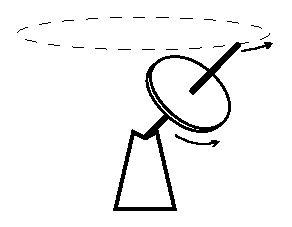
\includegraphics{figures/gyroscope}}
\caption{Schematic drawing of a gyroscope. The disc rapidly rotates about its own axis, and
    gravity causes a slower precession movement (shown as a dotted line) about a vertical axis.
    \label{gyroscope}}
\end{figure}

I set up initial conditions similar to the values one might find in a toy gyroscope (20
revolutions per second about the gyroscope axis, one full circle of precession in 8 seconds). I
then ran the simulation for 8~s, using an average time step length of about $2.3\cdot 10^{-4}$~s.
The simulation performed one full circle of precession in 7.953~s, which
is within 0.6~\% of the theoretical value. Over the course of 8~s, the body rotated by $320.36\pi$
radians about its own axis, which differs from the theoretical value by only 0.1~\%. These errors
varied little even in simulations using larger time steps. The effects of nutation\footnote{Having
nothing in common with \emph{mutation}, \emph{nutation} is an oscillation about an axis
orthogonal to the two main axes of rotation. \cite{Feynman:63}} were small for the chosen initial
conditions but may have contributed towards the errors.

It is interesting to also observe a different error, namely the amount by which the constraint
drifts apart. Usually this drift is compensated in the Lagrange multiplier method so that it
never manifests itself, but temporarily deactivating this
correction\footnote{by setting $k=d=0$ in equation~\ref{lagrangeEquation}.} makes the error
introduced by the ODE solver observable.

\begin{figure}
\centerline{% GNUPLOT: LaTeX picture with Postscript
\begingroup%
  \makeatletter%
  \newcommand{\GNUPLOTspecial}{%
    \@sanitize\catcode`\%=14\relax\special}%
  \setlength{\unitlength}{0.1bp}%
\begin{picture}(3600,2160)(0,0)%
{\GNUPLOTspecial{"
%!PS-Adobe-2.0 EPSF-2.0
%%Title: errorplot.tex
%%Creator: gnuplot 4.0 patchlevel 0
%%CreationDate: Mon Apr 17 12:02:25 2006
%%DocumentFonts: 
%%BoundingBox: 0 0 360 216
%%Orientation: Landscape
%%EndComments
/gnudict 256 dict def
gnudict begin
/Color false def
/Solid false def
/gnulinewidth 5.000 def
/userlinewidth gnulinewidth def
/vshift -33 def
/dl {10.0 mul} def
/hpt_ 31.5 def
/vpt_ 31.5 def
/hpt hpt_ def
/vpt vpt_ def
/Rounded false def
/M {moveto} bind def
/L {lineto} bind def
/R {rmoveto} bind def
/V {rlineto} bind def
/N {newpath moveto} bind def
/C {setrgbcolor} bind def
/f {rlineto fill} bind def
/vpt2 vpt 2 mul def
/hpt2 hpt 2 mul def
/Lshow { currentpoint stroke M
  0 vshift R show } def
/Rshow { currentpoint stroke M
  dup stringwidth pop neg vshift R show } def
/Cshow { currentpoint stroke M
  dup stringwidth pop -2 div vshift R show } def
/UP { dup vpt_ mul /vpt exch def hpt_ mul /hpt exch def
  /hpt2 hpt 2 mul def /vpt2 vpt 2 mul def } def
/DL { Color {setrgbcolor Solid {pop []} if 0 setdash }
 {pop pop pop 0 setgray Solid {pop []} if 0 setdash} ifelse } def
/BL { stroke userlinewidth 2 mul setlinewidth
      Rounded { 1 setlinejoin 1 setlinecap } if } def
/AL { stroke userlinewidth 2 div setlinewidth
      Rounded { 1 setlinejoin 1 setlinecap } if } def
/UL { dup gnulinewidth mul /userlinewidth exch def
      dup 1 lt {pop 1} if 10 mul /udl exch def } def
/PL { stroke userlinewidth setlinewidth
      Rounded { 1 setlinejoin 1 setlinecap } if } def
/LTw { PL [] 1 setgray } def
/LTb { BL [] 0 0 0 DL } def
/LTa { AL [1 udl mul 2 udl mul] 0 setdash 0 0 0 setrgbcolor } def
/LT0 { PL [] 1 0 0 DL } def
/LT1 { PL [4 dl 2 dl] 0 1 0 DL } def
/LT2 { PL [2 dl 3 dl] 0 0 1 DL } def
/LT3 { PL [1 dl 1.5 dl] 1 0 1 DL } def
/LT4 { PL [5 dl 2 dl 1 dl 2 dl] 0 1 1 DL } def
/LT5 { PL [4 dl 3 dl 1 dl 3 dl] 1 1 0 DL } def
/LT6 { PL [2 dl 2 dl 2 dl 4 dl] 0 0 0 DL } def
/LT7 { PL [2 dl 2 dl 2 dl 2 dl 2 dl 4 dl] 1 0.3 0 DL } def
/LT8 { PL [2 dl 2 dl 2 dl 2 dl 2 dl 2 dl 2 dl 4 dl] 0.5 0.5 0.5 DL } def
/Pnt { stroke [] 0 setdash
   gsave 1 setlinecap M 0 0 V stroke grestore } def
/Dia { stroke [] 0 setdash 2 copy vpt add M
  hpt neg vpt neg V hpt vpt neg V
  hpt vpt V hpt neg vpt V closepath stroke
  Pnt } def
/Pls { stroke [] 0 setdash vpt sub M 0 vpt2 V
  currentpoint stroke M
  hpt neg vpt neg R hpt2 0 V stroke
  } def
/Box { stroke [] 0 setdash 2 copy exch hpt sub exch vpt add M
  0 vpt2 neg V hpt2 0 V 0 vpt2 V
  hpt2 neg 0 V closepath stroke
  Pnt } def
/Crs { stroke [] 0 setdash exch hpt sub exch vpt add M
  hpt2 vpt2 neg V currentpoint stroke M
  hpt2 neg 0 R hpt2 vpt2 V stroke } def
/TriU { stroke [] 0 setdash 2 copy vpt 1.12 mul add M
  hpt neg vpt -1.62 mul V
  hpt 2 mul 0 V
  hpt neg vpt 1.62 mul V closepath stroke
  Pnt  } def
/Star { 2 copy Pls Crs } def
/BoxF { stroke [] 0 setdash exch hpt sub exch vpt add M
  0 vpt2 neg V  hpt2 0 V  0 vpt2 V
  hpt2 neg 0 V  closepath fill } def
/TriUF { stroke [] 0 setdash vpt 1.12 mul add M
  hpt neg vpt -1.62 mul V
  hpt 2 mul 0 V
  hpt neg vpt 1.62 mul V closepath fill } def
/TriD { stroke [] 0 setdash 2 copy vpt 1.12 mul sub M
  hpt neg vpt 1.62 mul V
  hpt 2 mul 0 V
  hpt neg vpt -1.62 mul V closepath stroke
  Pnt  } def
/TriDF { stroke [] 0 setdash vpt 1.12 mul sub M
  hpt neg vpt 1.62 mul V
  hpt 2 mul 0 V
  hpt neg vpt -1.62 mul V closepath fill} def
/DiaF { stroke [] 0 setdash vpt add M
  hpt neg vpt neg V hpt vpt neg V
  hpt vpt V hpt neg vpt V closepath fill } def
/Pent { stroke [] 0 setdash 2 copy gsave
  translate 0 hpt M 4 {72 rotate 0 hpt L} repeat
  closepath stroke grestore Pnt } def
/PentF { stroke [] 0 setdash gsave
  translate 0 hpt M 4 {72 rotate 0 hpt L} repeat
  closepath fill grestore } def
/Circle { stroke [] 0 setdash 2 copy
  hpt 0 360 arc stroke Pnt } def
/CircleF { stroke [] 0 setdash hpt 0 360 arc fill } def
/C0 { BL [] 0 setdash 2 copy moveto vpt 90 450  arc } bind def
/C1 { BL [] 0 setdash 2 copy        moveto
       2 copy  vpt 0 90 arc closepath fill
               vpt 0 360 arc closepath } bind def
/C2 { BL [] 0 setdash 2 copy moveto
       2 copy  vpt 90 180 arc closepath fill
               vpt 0 360 arc closepath } bind def
/C3 { BL [] 0 setdash 2 copy moveto
       2 copy  vpt 0 180 arc closepath fill
               vpt 0 360 arc closepath } bind def
/C4 { BL [] 0 setdash 2 copy moveto
       2 copy  vpt 180 270 arc closepath fill
               vpt 0 360 arc closepath } bind def
/C5 { BL [] 0 setdash 2 copy moveto
       2 copy  vpt 0 90 arc
       2 copy moveto
       2 copy  vpt 180 270 arc closepath fill
               vpt 0 360 arc } bind def
/C6 { BL [] 0 setdash 2 copy moveto
      2 copy  vpt 90 270 arc closepath fill
              vpt 0 360 arc closepath } bind def
/C7 { BL [] 0 setdash 2 copy moveto
      2 copy  vpt 0 270 arc closepath fill
              vpt 0 360 arc closepath } bind def
/C8 { BL [] 0 setdash 2 copy moveto
      2 copy vpt 270 360 arc closepath fill
              vpt 0 360 arc closepath } bind def
/C9 { BL [] 0 setdash 2 copy moveto
      2 copy  vpt 270 450 arc closepath fill
              vpt 0 360 arc closepath } bind def
/C10 { BL [] 0 setdash 2 copy 2 copy moveto vpt 270 360 arc closepath fill
       2 copy moveto
       2 copy vpt 90 180 arc closepath fill
               vpt 0 360 arc closepath } bind def
/C11 { BL [] 0 setdash 2 copy moveto
       2 copy  vpt 0 180 arc closepath fill
       2 copy moveto
       2 copy  vpt 270 360 arc closepath fill
               vpt 0 360 arc closepath } bind def
/C12 { BL [] 0 setdash 2 copy moveto
       2 copy  vpt 180 360 arc closepath fill
               vpt 0 360 arc closepath } bind def
/C13 { BL [] 0 setdash  2 copy moveto
       2 copy  vpt 0 90 arc closepath fill
       2 copy moveto
       2 copy  vpt 180 360 arc closepath fill
               vpt 0 360 arc closepath } bind def
/C14 { BL [] 0 setdash 2 copy moveto
       2 copy  vpt 90 360 arc closepath fill
               vpt 0 360 arc } bind def
/C15 { BL [] 0 setdash 2 copy vpt 0 360 arc closepath fill
               vpt 0 360 arc closepath } bind def
/Rec   { newpath 4 2 roll moveto 1 index 0 rlineto 0 exch rlineto
       neg 0 rlineto closepath } bind def
/Square { dup Rec } bind def
/Bsquare { vpt sub exch vpt sub exch vpt2 Square } bind def
/S0 { BL [] 0 setdash 2 copy moveto 0 vpt rlineto BL Bsquare } bind def
/S1 { BL [] 0 setdash 2 copy vpt Square fill Bsquare } bind def
/S2 { BL [] 0 setdash 2 copy exch vpt sub exch vpt Square fill Bsquare } bind def
/S3 { BL [] 0 setdash 2 copy exch vpt sub exch vpt2 vpt Rec fill Bsquare } bind def
/S4 { BL [] 0 setdash 2 copy exch vpt sub exch vpt sub vpt Square fill Bsquare } bind def
/S5 { BL [] 0 setdash 2 copy 2 copy vpt Square fill
       exch vpt sub exch vpt sub vpt Square fill Bsquare } bind def
/S6 { BL [] 0 setdash 2 copy exch vpt sub exch vpt sub vpt vpt2 Rec fill Bsquare } bind def
/S7 { BL [] 0 setdash 2 copy exch vpt sub exch vpt sub vpt vpt2 Rec fill
       2 copy vpt Square fill
       Bsquare } bind def
/S8 { BL [] 0 setdash 2 copy vpt sub vpt Square fill Bsquare } bind def
/S9 { BL [] 0 setdash 2 copy vpt sub vpt vpt2 Rec fill Bsquare } bind def
/S10 { BL [] 0 setdash 2 copy vpt sub vpt Square fill 2 copy exch vpt sub exch vpt Square fill
       Bsquare } bind def
/S11 { BL [] 0 setdash 2 copy vpt sub vpt Square fill 2 copy exch vpt sub exch vpt2 vpt Rec fill
       Bsquare } bind def
/S12 { BL [] 0 setdash 2 copy exch vpt sub exch vpt sub vpt2 vpt Rec fill Bsquare } bind def
/S13 { BL [] 0 setdash 2 copy exch vpt sub exch vpt sub vpt2 vpt Rec fill
       2 copy vpt Square fill Bsquare } bind def
/S14 { BL [] 0 setdash 2 copy exch vpt sub exch vpt sub vpt2 vpt Rec fill
       2 copy exch vpt sub exch vpt Square fill Bsquare } bind def
/S15 { BL [] 0 setdash 2 copy Bsquare fill Bsquare } bind def
/D0 { gsave translate 45 rotate 0 0 S0 stroke grestore } bind def
/D1 { gsave translate 45 rotate 0 0 S1 stroke grestore } bind def
/D2 { gsave translate 45 rotate 0 0 S2 stroke grestore } bind def
/D3 { gsave translate 45 rotate 0 0 S3 stroke grestore } bind def
/D4 { gsave translate 45 rotate 0 0 S4 stroke grestore } bind def
/D5 { gsave translate 45 rotate 0 0 S5 stroke grestore } bind def
/D6 { gsave translate 45 rotate 0 0 S6 stroke grestore } bind def
/D7 { gsave translate 45 rotate 0 0 S7 stroke grestore } bind def
/D8 { gsave translate 45 rotate 0 0 S8 stroke grestore } bind def
/D9 { gsave translate 45 rotate 0 0 S9 stroke grestore } bind def
/D10 { gsave translate 45 rotate 0 0 S10 stroke grestore } bind def
/D11 { gsave translate 45 rotate 0 0 S11 stroke grestore } bind def
/D12 { gsave translate 45 rotate 0 0 S12 stroke grestore } bind def
/D13 { gsave translate 45 rotate 0 0 S13 stroke grestore } bind def
/D14 { gsave translate 45 rotate 0 0 S14 stroke grestore } bind def
/D15 { gsave translate 45 rotate 0 0 S15 stroke grestore } bind def
/DiaE { stroke [] 0 setdash vpt add M
  hpt neg vpt neg V hpt vpt neg V
  hpt vpt V hpt neg vpt V closepath stroke } def
/BoxE { stroke [] 0 setdash exch hpt sub exch vpt add M
  0 vpt2 neg V hpt2 0 V 0 vpt2 V
  hpt2 neg 0 V closepath stroke } def
/TriUE { stroke [] 0 setdash vpt 1.12 mul add M
  hpt neg vpt -1.62 mul V
  hpt 2 mul 0 V
  hpt neg vpt 1.62 mul V closepath stroke } def
/TriDE { stroke [] 0 setdash vpt 1.12 mul sub M
  hpt neg vpt 1.62 mul V
  hpt 2 mul 0 V
  hpt neg vpt -1.62 mul V closepath stroke } def
/PentE { stroke [] 0 setdash gsave
  translate 0 hpt M 4 {72 rotate 0 hpt L} repeat
  closepath stroke grestore } def
/CircE { stroke [] 0 setdash 
  hpt 0 360 arc stroke } def
/Opaque { gsave closepath 1 setgray fill grestore 0 setgray closepath } def
/DiaW { stroke [] 0 setdash vpt add M
  hpt neg vpt neg V hpt vpt neg V
  hpt vpt V hpt neg vpt V Opaque stroke } def
/BoxW { stroke [] 0 setdash exch hpt sub exch vpt add M
  0 vpt2 neg V hpt2 0 V 0 vpt2 V
  hpt2 neg 0 V Opaque stroke } def
/TriUW { stroke [] 0 setdash vpt 1.12 mul add M
  hpt neg vpt -1.62 mul V
  hpt 2 mul 0 V
  hpt neg vpt 1.62 mul V Opaque stroke } def
/TriDW { stroke [] 0 setdash vpt 1.12 mul sub M
  hpt neg vpt 1.62 mul V
  hpt 2 mul 0 V
  hpt neg vpt -1.62 mul V Opaque stroke } def
/PentW { stroke [] 0 setdash gsave
  translate 0 hpt M 4 {72 rotate 0 hpt L} repeat
  Opaque stroke grestore } def
/CircW { stroke [] 0 setdash 
  hpt 0 360 arc Opaque stroke } def
/BoxFill { gsave Rec 1 setgray fill grestore } def
/BoxColFill {
  gsave Rec
  /Fillden exch def
  currentrgbcolor
  /ColB exch def /ColG exch def /ColR exch def
  /ColR ColR Fillden mul Fillden sub 1 add def
  /ColG ColG Fillden mul Fillden sub 1 add def
  /ColB ColB Fillden mul Fillden sub 1 add def
  ColR ColG ColB setrgbcolor
  fill grestore } def
%
% PostScript Level 1 Pattern Fill routine
% Usage: x y w h s a XX PatternFill
%	x,y = lower left corner of box to be filled
%	w,h = width and height of box
%	  a = angle in degrees between lines and x-axis
%	 XX = 0/1 for no/yes cross-hatch
%
/PatternFill { gsave /PFa [ 9 2 roll ] def
    PFa 0 get PFa 2 get 2 div add PFa 1 get PFa 3 get 2 div add translate
    PFa 2 get -2 div PFa 3 get -2 div PFa 2 get PFa 3 get Rec
    gsave 1 setgray fill grestore clip
    currentlinewidth 0.5 mul setlinewidth
    /PFs PFa 2 get dup mul PFa 3 get dup mul add sqrt def
    0 0 M PFa 5 get rotate PFs -2 div dup translate
	0 1 PFs PFa 4 get div 1 add floor cvi
	{ PFa 4 get mul 0 M 0 PFs V } for
    0 PFa 6 get ne {
	0 1 PFs PFa 4 get div 1 add floor cvi
	{ PFa 4 get mul 0 2 1 roll M PFs 0 V } for
    } if
    stroke grestore } def
%
/Symbol-Oblique /Symbol findfont [1 0 .167 1 0 0] makefont
dup length dict begin {1 index /FID eq {pop pop} {def} ifelse} forall
currentdict end definefont pop
end
%%EndProlog
gnudict begin
gsave
0 0 translate
0.100 0.100 scale
0 setgray
newpath
1.000 UL
LTb
550 300 M
31 0 V
1821 0 R
-31 0 V
550 393 M
63 0 V
1789 0 R
-63 0 V
1.000 UL
LTb
550 485 M
31 0 V
1821 0 R
-31 0 V
550 578 M
63 0 V
1789 0 R
-63 0 V
1.000 UL
LTb
550 671 M
31 0 V
1821 0 R
-31 0 V
550 763 M
63 0 V
1789 0 R
-63 0 V
1.000 UL
LTb
550 856 M
31 0 V
1821 0 R
-31 0 V
550 948 M
63 0 V
1789 0 R
-63 0 V
1.000 UL
LTb
550 1041 M
31 0 V
1821 0 R
-31 0 V
550 1134 M
63 0 V
1789 0 R
-63 0 V
1.000 UL
LTb
550 1226 M
31 0 V
1821 0 R
-31 0 V
550 1319 M
63 0 V
1789 0 R
-63 0 V
1.000 UL
LTb
550 1412 M
31 0 V
1821 0 R
-31 0 V
550 1504 M
63 0 V
1789 0 R
-63 0 V
1.000 UL
LTb
550 1597 M
31 0 V
1821 0 R
-31 0 V
550 1689 M
63 0 V
1789 0 R
-63 0 V
1.000 UL
LTb
550 1782 M
31 0 V
1821 0 R
-31 0 V
550 1875 M
63 0 V
1789 0 R
-63 0 V
1.000 UL
LTb
550 1967 M
31 0 V
1821 0 R
-31 0 V
550 2060 M
63 0 V
1789 0 R
-63 0 V
1.000 UL
LTb
550 300 M
0 63 V
0 1697 R
0 -63 V
1.000 UL
LTb
689 300 M
0 31 V
0 1729 R
0 -31 V
771 300 M
0 31 V
0 1729 R
0 -31 V
829 300 M
0 31 V
0 1729 R
0 -31 V
874 300 M
0 31 V
0 1729 R
0 -31 V
910 300 M
0 31 V
0 1729 R
0 -31 V
941 300 M
0 31 V
0 1729 R
0 -31 V
968 300 M
0 31 V
0 1729 R
0 -31 V
992 300 M
0 31 V
0 1729 R
0 -31 V
1013 300 M
0 63 V
0 1697 R
0 -63 V
1.000 UL
LTb
1152 300 M
0 31 V
0 1729 R
0 -31 V
1234 300 M
0 31 V
0 1729 R
0 -31 V
1292 300 M
0 31 V
0 1729 R
0 -31 V
1337 300 M
0 31 V
0 1729 R
0 -31 V
1373 300 M
0 31 V
0 1729 R
0 -31 V
1404 300 M
0 31 V
0 1729 R
0 -31 V
1431 300 M
0 31 V
0 1729 R
0 -31 V
1455 300 M
0 31 V
0 1729 R
0 -31 V
1476 300 M
0 63 V
0 1697 R
0 -63 V
1.000 UL
LTb
1615 300 M
0 31 V
0 1729 R
0 -31 V
1697 300 M
0 31 V
0 1729 R
0 -31 V
1755 300 M
0 31 V
0 1729 R
0 -31 V
1800 300 M
0 31 V
0 1729 R
0 -31 V
1836 300 M
0 31 V
0 1729 R
0 -31 V
1867 300 M
0 31 V
0 1729 R
0 -31 V
1894 300 M
0 31 V
0 1729 R
0 -31 V
1918 300 M
0 31 V
0 1729 R
0 -31 V
1939 300 M
0 63 V
0 1697 R
0 -63 V
1.000 UL
LTb
2078 300 M
0 31 V
0 1729 R
0 -31 V
2160 300 M
0 31 V
0 1729 R
0 -31 V
2218 300 M
0 31 V
0 1729 R
0 -31 V
2263 300 M
0 31 V
0 1729 R
0 -31 V
2299 300 M
0 31 V
0 1729 R
0 -31 V
2330 300 M
0 31 V
0 1729 R
0 -31 V
2357 300 M
0 31 V
0 1729 R
0 -31 V
2381 300 M
0 31 V
0 1729 R
0 -31 V
2402 300 M
0 63 V
0 1697 R
0 -63 V
1.000 UL
LTb
1.000 UL
LTb
550 300 M
1852 0 V
0 1760 V
-1852 0 V
550 300 L
LTb
LTb
1.000 UP
1.000 UP
1.000 UL
LT0
LTb
LT0
650 1869 M
263 0 V
1224 -87 R
-57 -93 V
-73 -92 V
-85 -93 V
-89 -92 V
-92 -93 V
-93 -93 V
-92 -92 V
-93 -93 V
-93 -93 V
-92 -92 V
-93 -93 V
-92 -92 V
-93 -93 V
908 485 L
815 393 L
2137 1782 Pls
2080 1689 Pls
2007 1597 Pls
1922 1504 Pls
1833 1412 Pls
1741 1319 Pls
1648 1226 Pls
1556 1134 Pls
1463 1041 Pls
1370 948 Pls
1278 856 Pls
1185 763 Pls
1093 671 Pls
1000 578 Pls
908 485 Pls
815 393 Pls
782 1869 Pls
1.000 UP
1.000 UL
LT1
LTb
LT1
650 1712 M
263 0 V
1224 285 R
-57 -146 V
-73 -94 V
-85 -94 V
-89 -91 V
-92 -93 V
-93 -93 V
-92 -91 V
-93 -37 V
-93 -65 V
-92 -71 V
-93 12 V
-92 -23 V
1000 995 L
-92 33 V
815 971 L
2137 1997 Crs
2080 1851 Crs
2007 1757 Crs
1922 1663 Crs
1833 1572 Crs
1741 1479 Crs
1648 1386 Crs
1556 1295 Crs
1463 1258 Crs
1370 1193 Crs
1278 1122 Crs
1185 1134 Crs
1093 1111 Crs
1000 995 Crs
908 1028 Crs
815 971 Crs
782 1712 Crs
1.000 UL
LTb
550 300 M
1852 0 V
0 1760 V
-1852 0 V
550 300 L
1.000 UP
stroke
grestore
end
showpage
}}%
\put(963,1712){\makebox(0,0)[l]{error over 8 sec}}%
\put(963,1869){\makebox(0,0)[l]{error per step}}%
\put(1476,50){\makebox(0,0){time step length}}%
\put(100,1180){%
\special{ps: gsave currentpoint currentpoint translate
270 rotate neg exch neg exch translate}%
\makebox(0,0)[b]{\shortstack{error}}%
\special{ps: currentpoint grestore moveto}%
}%
\put(2402,200){\makebox(0,0){ 0.1}}%
\put(1939,200){\makebox(0,0){ 0.01}}%
\put(1476,200){\makebox(0,0){ 0.001}}%
\put(1013,200){\makebox(0,0){ 1e-04}}%
\put(550,200){\makebox(0,0){ 1e-05}}%
\put(500,2060){\makebox(0,0)[r]{ 100}}%
\put(500,1875){\makebox(0,0)[r]{ 1}}%
\put(500,1689){\makebox(0,0)[r]{ 0.01}}%
\put(500,1504){\makebox(0,0)[r]{ 1e-04}}%
\put(500,1319){\makebox(0,0)[r]{ 1e-06}}%
\put(500,1134){\makebox(0,0)[r]{ 1e-08}}%
\put(500,948){\makebox(0,0)[r]{ 1e-10}}%
\put(500,763){\makebox(0,0)[r]{ 1e-12}}%
\put(500,578){\makebox(0,0)[r]{ 1e-14}}%
\put(500,393){\makebox(0,0)[r]{ 1e-16}}%
\end{picture}%
\endgroup
\endinput
}
\caption{Errors introduced by the ODE solver for different step sizes $h$, as observed in the
    gyroscope simulation.
    Solid line: difference between $O(h^4)$ and $O(h^5)$ Runge-Kutta approximations for each time
    step. Dashed line: cumulative drift of the gyroscope's `nail' constraint after 8~s simulation
    time.\label{errorplot}}
\end{figure}

Figure~\ref{errorplot} shows by what distance the gyroscope's `nail' constraint drifted apart
after 8~s of simulation time, for a wide range of different step sizes. There are some noteworthy
features about this plot:

\begin{itemize}
\item The logarithmic axes are scaled such that one order of magnitude in the horizontal has the
    same length as five orders of magnitude in the vertical. Observe that in this scaling, the
    solid line (error per time step) is an almost perfect straight line with gradient~1. This
    shows that the error is indeed an $O(h^5)$ function of the step size, as expected.
\item Over a wide range of step sizes, the plot of the total accumulated error is parallel to the
    solid line. This means the total error is also $O(h^5)$, which is even better than
    expected: although the approximation in each time step is $O(h^5)$, the number of steps
    required is inversely proportional to the step length, so one might expect a larger overall
    error. This relationship indicates that the ODE solver's target error can in fact be used
    as a reliable estimate of the overall error to within a constant factor.
\item As step sizes $h$ become very small~-- below about $3\cdot 10^{-4}$~s~-- the error in each
    step continues to scale order $O(h^5)$, but due to the huge number of steps, the accumulated
    error cannot be reduced much further. However, the errors here are in the range of nanometres,
    so they should be of little concern for computer graphics purposes.
\end{itemize}

In summary, the results for the simple gyroscope simulation inspire confidence that the
implementation is reliable and will continue to produce realistic results for complicated systems
which lack an exact solution. They also show that the target error can conveniently be adjusted
to match the requirements, because more CPU time does~-- within sensible bounds~-- buy higher
accuracy.


\subsection{Collision handling\label{evalCollisions}}

The analysis in the last section is relevant for continuous systems, but says nothing about
simulations involving collisions. For this purpose I simulated a different kind of physics toy,
\emph{Newton's cradle} (figure~\ref{cradleFigure}). This system does not have an exact analytical
solution, but it does have characteristic behaviour patterns which may be observed.

\begin{figure}
\centerline{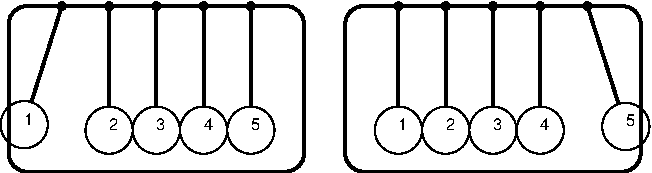
\includegraphics{figures/cradle}}
\caption{Newton's cradle. By conservation of momentum and energy, if $k$ balls collide with one
    end of the chain of balls, the same number of balls bounce up on the opposite side. The other
    balls stay stationary.\label{cradleFigure}}
\end{figure}

Newton's cradle works best when the elasticity is large ($\varepsilon \approx 1$). I simulated
it using $\varepsilon = 1.0$ and $\varepsilon = 0.9$, with one ball initially raised and the other
four at rest. The comparison of the two simulation results is shown in figure~\ref{cradlePlots}.
The energy is calculated as the sum of potential, linear and angular kinetic energies of all five
balls, with zero potential when all balls are at their equilibrium position. Fully elastic
collisions conserve energy in the simulation (constant to within $1$ part in $10^8$), while
imperfect collisions instantaneously dissipate energy.

The momentum of balls 2--4 stays zero (within $1$ part in $10^{10}$, except for transient peaks,
which are immediately neutralized again) with full elasticity; with $\varepsilon = 0.9$, they
increasingly begin to swing, as expected. The bottommost plots in figure~\ref{cradlePlots}
show how the step size is reduced to find the exact time of collision, and large time steps
are taken otherwise.

\begin{figure}
\centerline{% GNUPLOT: LaTeX picture with Postscript
\begingroup%
  \makeatletter%
  \newcommand{\GNUPLOTspecial}{%
    \@sanitize\catcode`\%=14\relax\special}%
  \setlength{\unitlength}{0.1bp}%
\begin{picture}(3239,5184)(0,0)%
{\GNUPLOTspecial{"
%!PS-Adobe-2.0 EPSF-2.0
%%Title: cradle.tex
%%Creator: gnuplot 4.0 patchlevel 0
%%CreationDate: Tue Apr 25 00:44:26 2006
%%DocumentFonts: 
%%BoundingBox: 0 0 323 518
%%Orientation: Landscape
%%EndComments
/gnudict 256 dict def
gnudict begin
/Color false def
/Solid false def
/gnulinewidth 5.000 def
/userlinewidth gnulinewidth def
/vshift -33 def
/dl {10.0 mul} def
/hpt_ 31.5 def
/vpt_ 31.5 def
/hpt hpt_ def
/vpt vpt_ def
/Rounded false def
/M {moveto} bind def
/L {lineto} bind def
/R {rmoveto} bind def
/V {rlineto} bind def
/N {newpath moveto} bind def
/C {setrgbcolor} bind def
/f {rlineto fill} bind def
/vpt2 vpt 2 mul def
/hpt2 hpt 2 mul def
/Lshow { currentpoint stroke M
  0 vshift R show } def
/Rshow { currentpoint stroke M
  dup stringwidth pop neg vshift R show } def
/Cshow { currentpoint stroke M
  dup stringwidth pop -2 div vshift R show } def
/UP { dup vpt_ mul /vpt exch def hpt_ mul /hpt exch def
  /hpt2 hpt 2 mul def /vpt2 vpt 2 mul def } def
/DL { Color {setrgbcolor Solid {pop []} if 0 setdash }
 {pop pop pop 0 setgray Solid {pop []} if 0 setdash} ifelse } def
/BL { stroke userlinewidth 2 mul setlinewidth
      Rounded { 1 setlinejoin 1 setlinecap } if } def
/AL { stroke userlinewidth 2 div setlinewidth
      Rounded { 1 setlinejoin 1 setlinecap } if } def
/UL { dup gnulinewidth mul /userlinewidth exch def
      dup 1 lt {pop 1} if 10 mul /udl exch def } def
/PL { stroke userlinewidth setlinewidth
      Rounded { 1 setlinejoin 1 setlinecap } if } def
/LTw { PL [] 1 setgray } def
/LTb { BL [] 0 0 0 DL } def
/LTa { AL [1 udl mul 2 udl mul] 0 setdash 0 0 0 setrgbcolor } def
/LT0 { PL [] 1 0 0 DL } def
/LT1 { PL [4 dl 2 dl] 0 1 0 DL } def
/LT2 { PL [2 dl 3 dl] 0 0 1 DL } def
/LT3 { PL [1 dl 1.5 dl] 1 0 1 DL } def
/LT4 { PL [5 dl 2 dl 1 dl 2 dl] 0 1 1 DL } def
/LT5 { PL [4 dl 3 dl 1 dl 3 dl] 1 1 0 DL } def
/LT6 { PL [2 dl 2 dl 2 dl 4 dl] 0 0 0 DL } def
/LT7 { PL [2 dl 2 dl 2 dl 2 dl 2 dl 4 dl] 1 0.3 0 DL } def
/LT8 { PL [2 dl 2 dl 2 dl 2 dl 2 dl 2 dl 2 dl 4 dl] 0.5 0.5 0.5 DL } def
/Pnt { stroke [] 0 setdash
   gsave 1 setlinecap M 0 0 V stroke grestore } def
/Dia { stroke [] 0 setdash 2 copy vpt add M
  hpt neg vpt neg V hpt vpt neg V
  hpt vpt V hpt neg vpt V closepath stroke
  Pnt } def
/Pls { stroke [] 0 setdash vpt sub M 0 vpt2 V
  currentpoint stroke M
  hpt neg vpt neg R hpt2 0 V stroke
  } def
/Box { stroke [] 0 setdash 2 copy exch hpt sub exch vpt add M
  0 vpt2 neg V hpt2 0 V 0 vpt2 V
  hpt2 neg 0 V closepath stroke
  Pnt } def
/Crs { stroke [] 0 setdash exch hpt sub exch vpt add M
  hpt2 vpt2 neg V currentpoint stroke M
  hpt2 neg 0 R hpt2 vpt2 V stroke } def
/TriU { stroke [] 0 setdash 2 copy vpt 1.12 mul add M
  hpt neg vpt -1.62 mul V
  hpt 2 mul 0 V
  hpt neg vpt 1.62 mul V closepath stroke
  Pnt  } def
/Star { 2 copy Pls Crs } def
/BoxF { stroke [] 0 setdash exch hpt sub exch vpt add M
  0 vpt2 neg V  hpt2 0 V  0 vpt2 V
  hpt2 neg 0 V  closepath fill } def
/TriUF { stroke [] 0 setdash vpt 1.12 mul add M
  hpt neg vpt -1.62 mul V
  hpt 2 mul 0 V
  hpt neg vpt 1.62 mul V closepath fill } def
/TriD { stroke [] 0 setdash 2 copy vpt 1.12 mul sub M
  hpt neg vpt 1.62 mul V
  hpt 2 mul 0 V
  hpt neg vpt -1.62 mul V closepath stroke
  Pnt  } def
/TriDF { stroke [] 0 setdash vpt 1.12 mul sub M
  hpt neg vpt 1.62 mul V
  hpt 2 mul 0 V
  hpt neg vpt -1.62 mul V closepath fill} def
/DiaF { stroke [] 0 setdash vpt add M
  hpt neg vpt neg V hpt vpt neg V
  hpt vpt V hpt neg vpt V closepath fill } def
/Pent { stroke [] 0 setdash 2 copy gsave
  translate 0 hpt M 4 {72 rotate 0 hpt L} repeat
  closepath stroke grestore Pnt } def
/PentF { stroke [] 0 setdash gsave
  translate 0 hpt M 4 {72 rotate 0 hpt L} repeat
  closepath fill grestore } def
/Circle { stroke [] 0 setdash 2 copy
  hpt 0 360 arc stroke Pnt } def
/CircleF { stroke [] 0 setdash hpt 0 360 arc fill } def
/C0 { BL [] 0 setdash 2 copy moveto vpt 90 450  arc } bind def
/C1 { BL [] 0 setdash 2 copy        moveto
       2 copy  vpt 0 90 arc closepath fill
               vpt 0 360 arc closepath } bind def
/C2 { BL [] 0 setdash 2 copy moveto
       2 copy  vpt 90 180 arc closepath fill
               vpt 0 360 arc closepath } bind def
/C3 { BL [] 0 setdash 2 copy moveto
       2 copy  vpt 0 180 arc closepath fill
               vpt 0 360 arc closepath } bind def
/C4 { BL [] 0 setdash 2 copy moveto
       2 copy  vpt 180 270 arc closepath fill
               vpt 0 360 arc closepath } bind def
/C5 { BL [] 0 setdash 2 copy moveto
       2 copy  vpt 0 90 arc
       2 copy moveto
       2 copy  vpt 180 270 arc closepath fill
               vpt 0 360 arc } bind def
/C6 { BL [] 0 setdash 2 copy moveto
      2 copy  vpt 90 270 arc closepath fill
              vpt 0 360 arc closepath } bind def
/C7 { BL [] 0 setdash 2 copy moveto
      2 copy  vpt 0 270 arc closepath fill
              vpt 0 360 arc closepath } bind def
/C8 { BL [] 0 setdash 2 copy moveto
      2 copy vpt 270 360 arc closepath fill
              vpt 0 360 arc closepath } bind def
/C9 { BL [] 0 setdash 2 copy moveto
      2 copy  vpt 270 450 arc closepath fill
              vpt 0 360 arc closepath } bind def
/C10 { BL [] 0 setdash 2 copy 2 copy moveto vpt 270 360 arc closepath fill
       2 copy moveto
       2 copy vpt 90 180 arc closepath fill
               vpt 0 360 arc closepath } bind def
/C11 { BL [] 0 setdash 2 copy moveto
       2 copy  vpt 0 180 arc closepath fill
       2 copy moveto
       2 copy  vpt 270 360 arc closepath fill
               vpt 0 360 arc closepath } bind def
/C12 { BL [] 0 setdash 2 copy moveto
       2 copy  vpt 180 360 arc closepath fill
               vpt 0 360 arc closepath } bind def
/C13 { BL [] 0 setdash  2 copy moveto
       2 copy  vpt 0 90 arc closepath fill
       2 copy moveto
       2 copy  vpt 180 360 arc closepath fill
               vpt 0 360 arc closepath } bind def
/C14 { BL [] 0 setdash 2 copy moveto
       2 copy  vpt 90 360 arc closepath fill
               vpt 0 360 arc } bind def
/C15 { BL [] 0 setdash 2 copy vpt 0 360 arc closepath fill
               vpt 0 360 arc closepath } bind def
/Rec   { newpath 4 2 roll moveto 1 index 0 rlineto 0 exch rlineto
       neg 0 rlineto closepath } bind def
/Square { dup Rec } bind def
/Bsquare { vpt sub exch vpt sub exch vpt2 Square } bind def
/S0 { BL [] 0 setdash 2 copy moveto 0 vpt rlineto BL Bsquare } bind def
/S1 { BL [] 0 setdash 2 copy vpt Square fill Bsquare } bind def
/S2 { BL [] 0 setdash 2 copy exch vpt sub exch vpt Square fill Bsquare } bind def
/S3 { BL [] 0 setdash 2 copy exch vpt sub exch vpt2 vpt Rec fill Bsquare } bind def
/S4 { BL [] 0 setdash 2 copy exch vpt sub exch vpt sub vpt Square fill Bsquare } bind def
/S5 { BL [] 0 setdash 2 copy 2 copy vpt Square fill
       exch vpt sub exch vpt sub vpt Square fill Bsquare } bind def
/S6 { BL [] 0 setdash 2 copy exch vpt sub exch vpt sub vpt vpt2 Rec fill Bsquare } bind def
/S7 { BL [] 0 setdash 2 copy exch vpt sub exch vpt sub vpt vpt2 Rec fill
       2 copy vpt Square fill
       Bsquare } bind def
/S8 { BL [] 0 setdash 2 copy vpt sub vpt Square fill Bsquare } bind def
/S9 { BL [] 0 setdash 2 copy vpt sub vpt vpt2 Rec fill Bsquare } bind def
/S10 { BL [] 0 setdash 2 copy vpt sub vpt Square fill 2 copy exch vpt sub exch vpt Square fill
       Bsquare } bind def
/S11 { BL [] 0 setdash 2 copy vpt sub vpt Square fill 2 copy exch vpt sub exch vpt2 vpt Rec fill
       Bsquare } bind def
/S12 { BL [] 0 setdash 2 copy exch vpt sub exch vpt sub vpt2 vpt Rec fill Bsquare } bind def
/S13 { BL [] 0 setdash 2 copy exch vpt sub exch vpt sub vpt2 vpt Rec fill
       2 copy vpt Square fill Bsquare } bind def
/S14 { BL [] 0 setdash 2 copy exch vpt sub exch vpt sub vpt2 vpt Rec fill
       2 copy exch vpt sub exch vpt Square fill Bsquare } bind def
/S15 { BL [] 0 setdash 2 copy Bsquare fill Bsquare } bind def
/D0 { gsave translate 45 rotate 0 0 S0 stroke grestore } bind def
/D1 { gsave translate 45 rotate 0 0 S1 stroke grestore } bind def
/D2 { gsave translate 45 rotate 0 0 S2 stroke grestore } bind def
/D3 { gsave translate 45 rotate 0 0 S3 stroke grestore } bind def
/D4 { gsave translate 45 rotate 0 0 S4 stroke grestore } bind def
/D5 { gsave translate 45 rotate 0 0 S5 stroke grestore } bind def
/D6 { gsave translate 45 rotate 0 0 S6 stroke grestore } bind def
/D7 { gsave translate 45 rotate 0 0 S7 stroke grestore } bind def
/D8 { gsave translate 45 rotate 0 0 S8 stroke grestore } bind def
/D9 { gsave translate 45 rotate 0 0 S9 stroke grestore } bind def
/D10 { gsave translate 45 rotate 0 0 S10 stroke grestore } bind def
/D11 { gsave translate 45 rotate 0 0 S11 stroke grestore } bind def
/D12 { gsave translate 45 rotate 0 0 S12 stroke grestore } bind def
/D13 { gsave translate 45 rotate 0 0 S13 stroke grestore } bind def
/D14 { gsave translate 45 rotate 0 0 S14 stroke grestore } bind def
/D15 { gsave translate 45 rotate 0 0 S15 stroke grestore } bind def
/DiaE { stroke [] 0 setdash vpt add M
  hpt neg vpt neg V hpt vpt neg V
  hpt vpt V hpt neg vpt V closepath stroke } def
/BoxE { stroke [] 0 setdash exch hpt sub exch vpt add M
  0 vpt2 neg V hpt2 0 V 0 vpt2 V
  hpt2 neg 0 V closepath stroke } def
/TriUE { stroke [] 0 setdash vpt 1.12 mul add M
  hpt neg vpt -1.62 mul V
  hpt 2 mul 0 V
  hpt neg vpt 1.62 mul V closepath stroke } def
/TriDE { stroke [] 0 setdash vpt 1.12 mul sub M
  hpt neg vpt 1.62 mul V
  hpt 2 mul 0 V
  hpt neg vpt -1.62 mul V closepath stroke } def
/PentE { stroke [] 0 setdash gsave
  translate 0 hpt M 4 {72 rotate 0 hpt L} repeat
  closepath stroke grestore } def
/CircE { stroke [] 0 setdash 
  hpt 0 360 arc stroke } def
/Opaque { gsave closepath 1 setgray fill grestore 0 setgray closepath } def
/DiaW { stroke [] 0 setdash vpt add M
  hpt neg vpt neg V hpt vpt neg V
  hpt vpt V hpt neg vpt V Opaque stroke } def
/BoxW { stroke [] 0 setdash exch hpt sub exch vpt add M
  0 vpt2 neg V hpt2 0 V 0 vpt2 V
  hpt2 neg 0 V Opaque stroke } def
/TriUW { stroke [] 0 setdash vpt 1.12 mul add M
  hpt neg vpt -1.62 mul V
  hpt 2 mul 0 V
  hpt neg vpt 1.62 mul V Opaque stroke } def
/TriDW { stroke [] 0 setdash vpt 1.12 mul sub M
  hpt neg vpt 1.62 mul V
  hpt 2 mul 0 V
  hpt neg vpt -1.62 mul V Opaque stroke } def
/PentW { stroke [] 0 setdash gsave
  translate 0 hpt M 4 {72 rotate 0 hpt L} repeat
  Opaque stroke grestore } def
/CircW { stroke [] 0 setdash 
  hpt 0 360 arc Opaque stroke } def
/BoxFill { gsave Rec 1 setgray fill grestore } def
/BoxColFill {
  gsave Rec
  /Fillden exch def
  currentrgbcolor
  /ColB exch def /ColG exch def /ColR exch def
  /ColR ColR Fillden mul Fillden sub 1 add def
  /ColG ColG Fillden mul Fillden sub 1 add def
  /ColB ColB Fillden mul Fillden sub 1 add def
  ColR ColG ColB setrgbcolor
  fill grestore } def
%
% PostScript Level 1 Pattern Fill routine
% Usage: x y w h s a XX PatternFill
%	x,y = lower left corner of box to be filled
%	w,h = width and height of box
%	  a = angle in degrees between lines and x-axis
%	 XX = 0/1 for no/yes cross-hatch
%
/PatternFill { gsave /PFa [ 9 2 roll ] def
    PFa 0 get PFa 2 get 2 div add PFa 1 get PFa 3 get 2 div add translate
    PFa 2 get -2 div PFa 3 get -2 div PFa 2 get PFa 3 get Rec
    gsave 1 setgray fill grestore clip
    currentlinewidth 0.5 mul setlinewidth
    /PFs PFa 2 get dup mul PFa 3 get dup mul add sqrt def
    0 0 M PFa 5 get rotate PFs -2 div dup translate
	0 1 PFs PFa 4 get div 1 add floor cvi
	{ PFa 4 get mul 0 M 0 PFs V } for
    0 PFa 6 get ne {
	0 1 PFs PFa 4 get div 1 add floor cvi
	{ PFa 4 get mul 0 2 1 roll M PFs 0 V } for
    } if
    stroke grestore } def
%
/Symbol-Oblique /Symbol findfont [1 0 .167 1 0 0] makefont
dup length dict begin {1 index /FID eq {pop pop} {def} ifelse} forall
currentdict end definefont pop
end
%%EndProlog
gnudict begin
gsave
0 0 translate
0.100 0.100 scale
0 setgray
newpath
1.000 UL
LTb
1.000 UL
LTa
100 5076 M
1700 0 V
1.000 UL
LTb
100 5076 M
-63 0 V
1.000 UL
LTb
1.000 UL
LTa
100 4999 M
1700 0 V
1.000 UL
LTb
100 4999 M
-31 0 V
1.000 UL
LTa
100 4922 M
1700 0 V
1.000 UL
LTb
100 4922 M
-63 0 V
1.000 UL
LTb
1.000 UL
LTa
100 4845 M
1700 0 V
1.000 UL
LTb
100 4845 M
-31 0 V
1.000 UL
LTa
100 4767 M
1700 0 V
1.000 UL
LTb
100 4767 M
-63 0 V
1.000 UL
LTb
1.000 UL
LTa
100 4690 M
1700 0 V
1.000 UL
LTb
100 4690 M
-31 0 V
1.000 UL
LTa
100 4613 M
1700 0 V
1.000 UL
LTb
100 4613 M
-63 0 V
1.000 UL
LTb
1.000 UL
LTa
100 4536 M
1700 0 V
1.000 UL
LTb
100 4536 M
-31 0 V
1.000 UL
LTa
1575 4536 M
0 540 V
1.000 UL
LTb
1575 4536 M
0 -63 V
1.000 UL
LTb
1.000 UL
LTa
1248 4536 M
0 540 V
1.000 UL
LTb
1248 4536 M
0 -63 V
1.000 UL
LTb
1.000 UL
LTa
920 4536 M
0 540 V
1.000 UL
LTb
920 4536 M
0 -63 V
1.000 UL
LTb
1.000 UL
LTa
592 4536 M
0 540 V
1.000 UL
LTb
592 4536 M
0 -63 V
1.000 UL
LTb
1.000 UL
LTa
264 4536 M
0 540 V
1.000 UL
LTb
264 4536 M
0 -63 V
1.000 UL
LTb
1.000 UL
LTa
100 4536 M
0 540 V
1.000 UL
LTb
100 4536 M
0 -63 V
1.000 UL
LTb
1.000 UL
LTa
100 4613 M
1700 0 V
1.000 UL
LTb
100 4536 M
1700 0 V
0 540 V
-1700 0 V
0 -540 V
LTb
1.000 UP
1.000 UL
LT0
100 4960 M
11 -2 V
15 -8 V
15 -15 V
14 -22 V
15 -28 V
15 -32 V
13 -35 V
13 -35 V
12 -36 V
11 -35 V
11 -34 V
9 -29 V
8 -25 V
2 -10 V
0 -1 V
1 0 V
1 0 V
1 0 V
4 0 V
7 0 V
9 0 V
9 0 V
11 0 V
11 0 V
11 0 V
12 0 V
12 0 V
13 0 V
13 0 V
14 0 V
14 0 V
15 0 V
14 0 V
15 0 V
14 0 V
15 0 V
15 0 V
15 0 V
13 0 V
13 0 V
12 0 V
12 0 V
10 0 V
10 0 V
9 0 V
3 0 V
0 1 V
0 1 V
1 1 V
1 3 V
1 5 V
4 12 V
7 22 V
9 30 V
9 32 V
11 32 V
11 33 V
11 31 V
12 31 V
12 28 V
13 26 V
13 22 V
14 18 V
14 12 V
15 7 V
14 -1 V
15 -7 V
14 -14 V
15 -20 V
15 -26 V
15 -32 V
13 -35 V
13 -35 V
12 -36 V
12 -35 V
10 -34 V
10 -33 V
9 -25 V
3 -13 V
0 -1 V
1 0 V
1 0 V
1 0 V
4 0 V
7 0 V
9 0 V
10 0 V
10 0 V
11 0 V
11 0 V
12 0 V
12 0 V
13 0 V
13 0 V
14 0 V
14 0 V
15 0 V
14 0 V
15 0 V
15 0 V
14 0 V
15 0 V
15 0 V
13 0 V
stroke
1179 4613 M
13 0 V
12 0 V
12 0 V
10 0 V
10 0 V
9 0 V
3 0 V
0 1 V
0 1 V
1 1 V
1 3 V
1 5 V
4 12 V
7 22 V
9 30 V
9 32 V
11 32 V
11 32 V
11 32 V
12 31 V
12 28 V
13 26 V
13 22 V
14 18 V
14 12 V
15 7 V
14 -1 V
15 -7 V
14 -14 V
15 -20 V
15 -26 V
15 -32 V
13 -34 V
13 -36 V
12 -36 V
12 -35 V
10 -34 V
10 -33 V
9 -25 V
3 -13 V
0 -1 V
1 0 V
1 0 V
3 0 V
5 0 V
8 0 V
10 0 V
10 0 V
11 0 V
11 0 V
11 0 V
12 0 V
13 0 V
13 0 V
13 0 V
14 0 V
15 0 V
15 0 V
14 0 V
15 0 V
14 0 V
15 0 V
1.000 UL
LTb
100 4536 M
1700 0 V
0 540 V
-1700 0 V
0 -540 V
1.000 UP
1.000 UL
LTb
1.000 UL
LTa
100 4428 M
1700 0 V
1.000 UL
LTb
100 4428 M
-31 0 V
1.000 UL
LTa
100 4338 M
1700 0 V
1.000 UL
LTb
100 4338 M
-63 0 V
1.000 UL
LTb
1.000 UL
LTa
100 4248 M
1700 0 V
1.000 UL
LTb
100 4248 M
-31 0 V
1.000 UL
LTa
100 4158 M
1700 0 V
1.000 UL
LTb
100 4158 M
-63 0 V
1.000 UL
LTb
1.000 UL
LTa
100 4068 M
1700 0 V
1.000 UL
LTb
100 4068 M
-31 0 V
1.000 UL
LTa
100 3978 M
1700 0 V
1.000 UL
LTb
100 3978 M
-63 0 V
1.000 UL
LTb
1.000 UL
LTa
100 3888 M
1700 0 V
1.000 UL
LTb
100 3888 M
-31 0 V
1.000 UL
LTa
1575 3888 M
0 540 V
1.000 UL
LTb
1575 3888 M
0 -63 V
1.000 UL
LTb
1.000 UL
LTa
1248 3888 M
0 540 V
1.000 UL
LTb
1248 3888 M
0 -63 V
1.000 UL
LTb
1.000 UL
LTa
920 3888 M
0 540 V
1.000 UL
LTb
920 3888 M
0 -63 V
1.000 UL
LTb
1.000 UL
LTa
592 3888 M
0 540 V
1.000 UL
LTb
592 3888 M
0 -63 V
1.000 UL
LTb
1.000 UL
LTa
264 3888 M
0 540 V
1.000 UL
LTb
264 3888 M
0 -63 V
1.000 UL
LTb
1.000 UL
LTa
100 3888 M
0 540 V
1.000 UL
LTb
100 3888 M
0 -63 V
1.000 UL
LTb
1.000 UL
LTa
100 4158 M
1700 0 V
1.000 UL
LTb
100 3888 M
1700 0 V
0 540 V
-1700 0 V
0 -540 V
LTb
1.000 UP
1.000 UL
LT0
100 4158 M
11 0 V
15 0 V
15 0 V
14 0 V
15 0 V
15 0 V
13 0 V
13 0 V
12 0 V
11 0 V
11 0 V
9 0 V
8 0 V
2 0 V
1 0 V
1 0 V
1 0 V
4 0 V
7 0 V
9 0 V
9 0 V
11 0 V
11 0 V
11 0 V
12 0 V
12 0 V
13 0 V
13 0 V
14 0 V
14 0 V
15 0 V
14 0 V
15 0 V
14 0 V
15 0 V
15 0 V
15 0 V
13 0 V
13 0 V
12 0 V
12 0 V
10 0 V
10 0 V
9 0 V
3 0 V
1 0 V
1 0 V
1 0 V
4 0 V
7 0 V
9 0 V
9 0 V
11 0 V
11 0 V
11 0 V
12 0 V
12 0 V
13 0 V
13 0 V
14 0 V
14 0 V
15 0 V
14 0 V
15 0 V
14 0 V
15 0 V
15 0 V
15 0 V
13 0 V
13 0 V
12 0 V
12 0 V
10 0 V
10 0 V
9 0 V
3 0 V
1 0 V
1 0 V
1 0 V
4 0 V
7 0 V
9 0 V
10 0 V
10 0 V
11 0 V
11 0 V
12 0 V
12 0 V
13 0 V
13 0 V
14 0 V
14 0 V
15 0 V
14 0 V
15 0 V
15 0 V
14 0 V
15 0 V
15 0 V
13 0 V
13 0 V
12 0 V
12 0 V
10 0 V
stroke
1226 4158 M
10 0 V
9 0 V
3 0 V
1 0 V
1 0 V
1 0 V
4 0 V
7 0 V
9 0 V
9 0 V
11 0 V
11 0 V
11 0 V
12 0 V
12 0 V
13 0 V
13 0 V
14 0 V
14 0 V
15 0 V
14 0 V
15 0 V
14 0 V
15 0 V
15 0 V
15 0 V
13 0 V
13 0 V
12 0 V
12 0 V
10 0 V
10 0 V
9 0 V
3 0 V
1 0 V
1 0 V
3 0 V
5 0 V
8 0 V
10 0 V
10 0 V
11 0 V
11 0 V
11 0 V
12 0 V
13 0 V
13 0 V
13 0 V
14 0 V
15 0 V
15 0 V
14 0 V
15 0 V
14 0 V
15 0 V
1.000 UL
LTb
100 3888 M
1700 0 V
0 540 V
-1700 0 V
0 -540 V
1.000 UP
1.000 UL
LTb
1.000 UL
LTa
100 3780 M
1700 0 V
1.000 UL
LTb
100 3780 M
-31 0 V
1.000 UL
LTa
100 3703 M
1700 0 V
1.000 UL
LTb
100 3703 M
-63 0 V
1.000 UL
LTb
1.000 UL
LTa
100 3626 M
1700 0 V
1.000 UL
LTb
100 3626 M
-31 0 V
1.000 UL
LTa
100 3549 M
1700 0 V
1.000 UL
LTb
100 3549 M
-63 0 V
1.000 UL
LTb
1.000 UL
LTa
100 3471 M
1700 0 V
1.000 UL
LTb
100 3471 M
-31 0 V
1.000 UL
LTa
100 3394 M
1700 0 V
1.000 UL
LTb
100 3394 M
-63 0 V
1.000 UL
LTb
1.000 UL
LTa
100 3317 M
1700 0 V
1.000 UL
LTb
100 3317 M
-31 0 V
1.000 UL
LTa
100 3240 M
1700 0 V
1.000 UL
LTb
100 3240 M
-63 0 V
1.000 UL
LTb
1.000 UL
LTa
1575 3240 M
0 540 V
1.000 UL
LTb
1575 3240 M
0 -63 V
1.000 UL
LTb
1.000 UL
LTa
1248 3240 M
0 540 V
1.000 UL
LTb
1248 3240 M
0 -63 V
1.000 UL
LTb
1.000 UL
LTa
920 3240 M
0 540 V
1.000 UL
LTb
920 3240 M
0 -63 V
1.000 UL
LTb
1.000 UL
LTa
592 3240 M
0 540 V
1.000 UL
LTb
592 3240 M
0 -63 V
1.000 UL
LTb
1.000 UL
LTa
264 3240 M
0 540 V
1.000 UL
LTb
264 3240 M
0 -63 V
1.000 UL
LTb
1.000 UL
LTa
100 3240 M
0 540 V
1.000 UL
LTb
100 3240 M
0 -63 V
1.000 UL
LTb
1.000 UL
LTa
100 3703 M
1700 0 V
1.000 UL
LTb
100 3240 M
1700 0 V
0 540 V
-1700 0 V
0 -540 V
LTb
1.000 UP
1.000 UL
LT0
100 3703 M
11 0 V
15 0 V
15 0 V
14 0 V
15 0 V
15 0 V
13 0 V
13 0 V
12 0 V
11 0 V
11 0 V
9 0 V
8 0 V
2 0 V
0 -1 V
0 -1 V
1 -1 V
1 -3 V
1 -5 V
4 -12 V
7 -22 V
9 -30 V
9 -32 V
11 -32 V
11 -32 V
11 -32 V
12 -31 V
12 -28 V
13 -26 V
13 -22 V
14 -18 V
14 -12 V
15 -7 V
14 1 V
15 7 V
14 14 V
15 20 V
15 26 V
15 32 V
13 34 V
13 36 V
12 36 V
12 35 V
10 34 V
10 33 V
9 25 V
3 13 V
0 1 V
1 0 V
1 0 V
1 0 V
4 0 V
7 0 V
9 0 V
9 0 V
11 0 V
11 0 V
11 0 V
12 0 V
12 0 V
13 0 V
13 0 V
14 0 V
14 0 V
15 0 V
14 0 V
15 0 V
14 0 V
15 0 V
15 0 V
15 0 V
13 0 V
13 0 V
12 0 V
12 0 V
10 0 V
10 0 V
9 0 V
3 0 V
0 -1 V
0 -1 V
1 -1 V
1 -3 V
1 -5 V
4 -12 V
7 -22 V
9 -30 V
10 -32 V
10 -32 V
11 -33 V
11 -32 V
12 -30 V
12 -28 V
13 -26 V
13 -22 V
14 -18 V
14 -12 V
15 -7 V
14 1 V
15 7 V
15 14 V
14 20 V
15 27 V
15 31 V
stroke
1166 3456 M
13 35 V
13 35 V
12 36 V
12 35 V
10 35 V
10 32 V
9 25 V
3 13 V
0 1 V
1 0 V
1 0 V
1 0 V
4 0 V
7 0 V
9 0 V
9 0 V
11 0 V
11 0 V
11 0 V
12 0 V
12 0 V
13 0 V
13 0 V
14 0 V
14 0 V
15 0 V
14 0 V
15 0 V
14 0 V
15 0 V
15 0 V
15 0 V
13 0 V
13 0 V
12 0 V
12 0 V
10 0 V
10 0 V
9 0 V
3 0 V
0 -1 V
1 -1 V
0 -2 V
1 -4 V
3 -8 V
5 -16 V
8 -29 V
10 -31 V
10 -32 V
11 -32 V
11 -33 V
11 -31 V
12 -29 V
13 -27 V
13 -24 V
13 -20 V
14 -15 V
15 -10 V
15 -2 V
14 4 V
15 10 V
14 18 V
15 23 V
1.000 UL
LTb
100 3240 M
1700 0 V
0 540 V
-1700 0 V
0 -540 V
1.000 UP
1.000 UL
LTb
1.000 UL
LTa
100 3093 M
1700 0 V
1.000 UL
LTb
100 3093 M
-31 0 V
1.000 UL
LTa
100 3016 M
1700 0 V
1.000 UL
LTb
100 3016 M
-63 0 V
1.000 UL
LTb
1.000 UL
LTa
100 2939 M
1700 0 V
1.000 UL
LTb
100 2939 M
-31 0 V
1.000 UL
LTa
100 2862 M
1700 0 V
1.000 UL
LTb
100 2862 M
-63 0 V
1.000 UL
LTb
1.000 UL
LTa
100 2785 M
1700 0 V
1.000 UL
LTb
100 2785 M
-31 0 V
1.000 UL
LTa
100 2708 M
1700 0 V
1.000 UL
LTb
100 2708 M
-63 0 V
1.000 UL
LTb
1.000 UL
LTa
100 2631 M
1700 0 V
1.000 UL
LTb
100 2631 M
-31 0 V
1.000 UL
LTa
1575 2592 M
0 540 V
1.000 UL
LTb
1575 2592 M
0 -63 V
1.000 UL
LTb
1.000 UL
LTa
1248 2592 M
0 540 V
1.000 UL
LTb
1248 2592 M
0 -63 V
1.000 UL
LTb
1.000 UL
LTa
920 2592 M
0 540 V
1.000 UL
LTb
920 2592 M
0 -63 V
1.000 UL
LTb
1.000 UL
LTa
592 2592 M
0 540 V
1.000 UL
LTb
592 2592 M
0 -63 V
1.000 UL
LTb
1.000 UL
LTa
264 2592 M
0 540 V
1.000 UL
LTb
264 2592 M
0 -63 V
1.000 UL
LTb
1.000 UL
LTa
100 2592 M
0 540 V
1.000 UL
LTb
100 2592 M
0 -63 V
1.000 UL
LTb
1.000 UL
LTa
100 2862 M
1700 0 V
1.000 UL
LTb
100 2592 M
1700 0 V
0 540 V
-1700 0 V
0 -540 V
LTb
1.000 UP
1.000 UL
LT0
100 2862 M
11 24 V
15 30 V
15 30 V
14 29 V
15 28 V
15 25 V
13 21 V
13 17 V
12 14 V
11 10 V
11 6 V
9 3 V
8 2 V
2 0 V
0 -239 V
1 0 V
1 0 V
1 0 V
4 0 V
7 0 V
9 0 V
9 0 V
11 0 V
11 0 V
11 0 V
12 0 V
12 0 V
13 0 V
13 0 V
14 0 V
14 0 V
15 0 V
14 0 V
15 0 V
14 0 V
15 0 V
15 0 V
15 0 V
13 0 V
13 0 V
12 0 V
12 0 V
10 0 V
10 0 V
9 0 V
3 0 V
0 -239 V
1 0 V
1 0 V
1 0 V
4 1 V
7 1 V
9 5 V
9 6 V
11 10 V
11 12 V
11 16 V
12 18 V
12 21 V
13 23 V
13 25 V
14 28 V
14 29 V
15 31 V
14 30 V
15 31 V
14 30 V
15 29 V
15 28 V
15 26 V
13 22 V
13 18 V
12 14 V
12 11 V
10 7 V
10 4 V
9 2 V
3 0 V
0 -239 V
1 0 V
1 0 V
1 0 V
4 0 V
7 0 V
9 0 V
10 0 V
10 0 V
11 0 V
11 0 V
12 0 V
12 0 V
13 0 V
13 0 V
14 0 V
14 0 V
15 0 V
14 0 V
15 0 V
15 0 V
14 0 V
15 0 V
15 0 V
13 0 V
13 0 V
stroke
1192 2862 M
12 0 V
12 0 V
10 0 V
10 0 V
9 0 V
3 0 V
0 -239 V
1 0 V
1 0 V
1 0 V
4 1 V
7 1 V
9 5 V
9 6 V
11 10 V
11 12 V
11 16 V
12 18 V
12 21 V
13 23 V
13 25 V
14 28 V
14 29 V
15 31 V
14 30 V
15 31 V
14 30 V
15 29 V
15 28 V
15 26 V
13 22 V
13 18 V
12 14 V
12 11 V
10 7 V
10 4 V
9 2 V
3 0 V
0 -239 V
1 0 V
1 0 V
3 0 V
5 0 V
8 0 V
10 0 V
10 0 V
11 0 V
11 0 V
11 0 V
12 0 V
13 0 V
13 0 V
13 0 V
14 0 V
15 0 V
15 0 V
14 0 V
15 0 V
14 0 V
15 0 V
1.000 UL
LTb
100 2592 M
1700 0 V
0 540 V
-1700 0 V
0 -540 V
1.000 UP
1.000 UL
LTb
1.000 UL
LTa
100 2445 M
1700 0 V
1.000 UL
LTb
100 2445 M
-31 0 V
1.000 UL
LTa
100 2368 M
1700 0 V
1.000 UL
LTb
100 2368 M
-63 0 V
1.000 UL
LTb
1.000 UL
LTa
100 2291 M
1700 0 V
1.000 UL
LTb
100 2291 M
-31 0 V
1.000 UL
LTa
100 2214 M
1700 0 V
1.000 UL
LTb
100 2214 M
-63 0 V
1.000 UL
LTb
1.000 UL
LTa
100 2137 M
1700 0 V
1.000 UL
LTb
100 2137 M
-31 0 V
1.000 UL
LTa
100 2060 M
1700 0 V
1.000 UL
LTb
100 2060 M
-63 0 V
1.000 UL
LTb
1.000 UL
LTa
100 1983 M
1700 0 V
1.000 UL
LTb
100 1983 M
-31 0 V
1.000 UL
LTa
1575 1944 M
0 540 V
1.000 UL
LTb
1575 1944 M
0 -63 V
1.000 UL
LTb
1.000 UL
LTa
1248 1944 M
0 540 V
1.000 UL
LTb
1248 1944 M
0 -63 V
1.000 UL
LTb
1.000 UL
LTa
920 1944 M
0 540 V
1.000 UL
LTb
920 1944 M
0 -63 V
1.000 UL
LTb
1.000 UL
LTa
592 1944 M
0 540 V
1.000 UL
LTb
592 1944 M
0 -63 V
1.000 UL
LTb
1.000 UL
LTa
264 1944 M
0 540 V
1.000 UL
LTb
264 1944 M
0 -63 V
1.000 UL
LTb
1.000 UL
LTa
100 1944 M
0 540 V
1.000 UL
LTb
100 1944 M
0 -63 V
1.000 UL
LTb
1.000 UL
LTa
100 2214 M
1700 0 V
1.000 UL
LTb
100 1944 M
1700 0 V
0 540 V
-1700 0 V
0 -540 V
LTb
1.000 UP
1.000 UL
LT0
100 2214 M
11 0 V
15 0 V
15 0 V
14 0 V
15 0 V
15 0 V
13 0 V
13 0 V
12 0 V
11 0 V
11 0 V
9 0 V
8 0 V
2 0 V
0 239 V
0 -239 V
1 0 V
1 0 V
1 0 V
4 0 V
7 0 V
9 0 V
9 0 V
11 0 V
11 0 V
11 0 V
12 0 V
12 0 V
13 0 V
13 0 V
14 0 V
14 0 V
15 0 V
14 0 V
15 0 V
14 0 V
15 0 V
15 0 V
15 0 V
13 0 V
13 0 V
12 0 V
12 0 V
10 0 V
10 0 V
9 0 V
3 0 V
0 -239 V
0 239 V
1 0 V
1 0 V
1 0 V
4 0 V
7 0 V
9 0 V
9 0 V
11 0 V
11 0 V
11 0 V
12 0 V
12 0 V
13 0 V
13 0 V
14 0 V
14 0 V
15 0 V
14 0 V
15 0 V
14 0 V
15 0 V
15 0 V
15 0 V
13 0 V
13 0 V
12 0 V
12 0 V
10 0 V
10 0 V
9 0 V
3 0 V
0 239 V
0 -239 V
1 0 V
1 0 V
1 0 V
4 0 V
7 0 V
9 0 V
10 0 V
10 0 V
11 0 V
11 0 V
12 0 V
12 0 V
13 0 V
13 0 V
14 0 V
14 0 V
15 0 V
14 0 V
15 0 V
15 0 V
14 0 V
15 0 V
stroke
1151 2214 M
15 0 V
13 0 V
13 0 V
12 0 V
12 0 V
10 0 V
10 0 V
9 0 V
3 0 V
1 0 V
1 0 V
1 0 V
4 0 V
7 0 V
9 0 V
9 0 V
11 0 V
11 0 V
11 0 V
12 0 V
12 0 V
13 0 V
13 0 V
14 0 V
14 0 V
15 0 V
14 0 V
15 0 V
14 0 V
15 0 V
15 0 V
15 0 V
13 0 V
13 0 V
12 0 V
12 0 V
10 0 V
10 0 V
9 0 V
3 0 V
0 239 V
0 -239 V
1 0 V
1 0 V
3 0 V
5 0 V
8 0 V
10 0 V
10 0 V
11 0 V
11 0 V
11 0 V
12 0 V
13 0 V
13 0 V
13 0 V
14 0 V
15 0 V
15 0 V
14 0 V
15 0 V
14 0 V
15 0 V
1.000 UL
LTb
100 1944 M
1700 0 V
0 540 V
-1700 0 V
0 -540 V
1.000 UP
1.000 UL
LTb
1.000 UL
LTa
100 1797 M
1700 0 V
1.000 UL
LTb
100 1797 M
-31 0 V
1.000 UL
LTa
100 1720 M
1700 0 V
1.000 UL
LTb
100 1720 M
-63 0 V
1.000 UL
LTb
1.000 UL
LTa
100 1643 M
1700 0 V
1.000 UL
LTb
100 1643 M
-31 0 V
1.000 UL
LTa
100 1566 M
1700 0 V
1.000 UL
LTb
100 1566 M
-63 0 V
1.000 UL
LTb
1.000 UL
LTa
100 1489 M
1700 0 V
1.000 UL
LTb
100 1489 M
-31 0 V
1.000 UL
LTa
100 1412 M
1700 0 V
1.000 UL
LTb
100 1412 M
-63 0 V
1.000 UL
LTb
1.000 UL
LTa
100 1335 M
1700 0 V
1.000 UL
LTb
100 1335 M
-31 0 V
1.000 UL
LTa
1575 1296 M
0 540 V
1.000 UL
LTb
1575 1296 M
0 -63 V
1.000 UL
LTb
1.000 UL
LTa
1248 1296 M
0 540 V
1.000 UL
LTb
1248 1296 M
0 -63 V
1.000 UL
LTb
1.000 UL
LTa
920 1296 M
0 540 V
1.000 UL
LTb
920 1296 M
0 -63 V
1.000 UL
LTb
1.000 UL
LTa
592 1296 M
0 540 V
1.000 UL
LTb
592 1296 M
0 -63 V
1.000 UL
LTb
1.000 UL
LTa
264 1296 M
0 540 V
1.000 UL
LTb
264 1296 M
0 -63 V
1.000 UL
LTb
1.000 UL
LTa
100 1296 M
0 540 V
1.000 UL
LTb
100 1296 M
0 -63 V
1.000 UL
LTb
1.000 UL
LTa
100 1566 M
1700 0 V
1.000 UL
LTb
100 1296 M
1700 0 V
0 540 V
-1700 0 V
0 -540 V
LTb
1.000 UP
1.000 UL
LT0
100 1566 M
11 0 V
15 0 V
15 0 V
14 0 V
15 0 V
15 0 V
13 0 V
13 0 V
12 0 V
11 0 V
11 0 V
9 0 V
8 0 V
2 0 V
0 239 V
1 0 V
1 0 V
1 0 V
4 -1 V
7 -1 V
9 -5 V
9 -6 V
11 -10 V
11 -12 V
11 -16 V
12 -18 V
12 -21 V
13 -23 V
13 -25 V
14 -28 V
14 -29 V
15 -31 V
14 -30 V
15 -31 V
14 -30 V
15 -29 V
15 -28 V
15 -26 V
13 -22 V
13 -18 V
12 -14 V
12 -11 V
10 -7 V
10 -4 V
9 -2 V
3 0 V
0 239 V
1 0 V
1 0 V
1 0 V
4 0 V
7 0 V
9 0 V
9 0 V
11 0 V
11 0 V
11 0 V
12 0 V
12 0 V
13 0 V
13 0 V
14 0 V
14 0 V
15 0 V
14 0 V
15 0 V
14 0 V
15 0 V
15 0 V
15 0 V
13 0 V
13 0 V
12 0 V
12 0 V
10 0 V
10 0 V
9 0 V
3 0 V
0 239 V
1 0 V
1 0 V
1 0 V
4 -1 V
7 -1 V
9 -5 V
10 -6 V
10 -10 V
11 -13 V
11 -15 V
12 -18 V
12 -21 V
13 -23 V
13 -25 V
14 -28 V
14 -29 V
15 -31 V
14 -31 V
15 -30 V
15 -30 V
14 -29 V
15 -28 V
15 -26 V
13 -22 V
13 -18 V
stroke
1192 1365 M
12 -14 V
12 -11 V
10 -7 V
10 -4 V
9 -2 V
3 0 V
0 239 V
1 0 V
1 0 V
1 0 V
4 0 V
7 0 V
9 0 V
9 0 V
11 0 V
11 0 V
11 0 V
12 0 V
12 0 V
13 0 V
13 0 V
14 0 V
14 0 V
15 0 V
14 0 V
15 0 V
14 0 V
15 0 V
15 0 V
15 0 V
13 0 V
13 0 V
12 0 V
12 0 V
10 0 V
10 0 V
9 0 V
3 0 V
0 239 V
1 0 V
1 0 V
3 0 V
5 -1 V
8 -3 V
10 -6 V
10 -8 V
11 -11 V
11 -14 V
11 -17 V
12 -20 V
13 -22 V
13 -24 V
13 -27 V
14 -28 V
15 -30 V
15 -31 V
14 -30 V
15 -30 V
14 -30 V
15 -29 V
1.000 UL
LTb
100 1296 M
1700 0 V
0 540 V
-1700 0 V
0 -540 V
1.000 UP
1.000 UL
LTb
1.000 UL
LTa
100 1188 M
1700 0 V
1.000 UL
LTb
100 1188 M
-63 0 V
1.000 UL
LTb
1.000 UL
LTa
100 1053 M
1700 0 V
1.000 UL
LTb
100 1053 M
-63 0 V
1.000 UL
LTb
1.000 UL
LTa
100 918 M
1700 0 V
1.000 UL
LTb
100 918 M
-63 0 V
1.000 UL
LTb
1.000 UL
LTa
100 783 M
1700 0 V
1.000 UL
LTb
100 783 M
-63 0 V
1.000 UL
LTb
1.000 UL
LTa
100 648 M
1700 0 V
1.000 UL
LTb
100 648 M
-63 0 V
1.000 UL
LTb
1.000 UL
LTa
1575 648 M
0 540 V
1.000 UL
LTb
1575 648 M
0 -63 V
1.000 UL
LTb
1.000 UL
LTa
1248 648 M
0 540 V
1.000 UL
LTb
1248 648 M
0 -63 V
1.000 UL
LTb
1.000 UL
LTa
920 648 M
0 540 V
1.000 UL
LTb
920 648 M
0 -63 V
1.000 UL
LTb
1.000 UL
LTa
592 648 M
0 540 V
1.000 UL
LTb
592 648 M
0 -63 V
1.000 UL
LTb
1.000 UL
LTa
264 648 M
0 540 V
1.000 UL
LTb
264 648 M
0 -63 V
1.000 UL
LTb
1.000 UL
LTa
100 648 M
0 540 V
1.000 UL
LTb
100 648 M
0 -63 V
1.000 UL
LTb
1.000 UL
LTb
100 648 M
1700 0 V
0 540 V
-1700 0 V
0 -540 V
LTb
1.000 UP
1.000 UL
LT0
100 1132 M
11 0 V
15 0 V
15 0 V
14 0 V
15 0 V
15 0 V
13 0 V
13 0 V
12 0 V
11 0 V
11 0 V
9 0 V
8 0 V
2 0 V
1 0 V
1 0 V
1 0 V
4 0 V
7 0 V
9 0 V
9 0 V
11 0 V
11 0 V
11 0 V
12 0 V
12 0 V
13 0 V
13 0 V
14 0 V
14 0 V
15 0 V
14 0 V
15 0 V
14 0 V
15 0 V
15 0 V
15 0 V
13 0 V
13 0 V
12 0 V
12 0 V
10 0 V
10 0 V
9 0 V
3 0 V
1 0 V
1 0 V
1 0 V
4 0 V
7 0 V
9 0 V
9 0 V
11 0 V
11 0 V
11 0 V
12 0 V
12 0 V
13 0 V
13 0 V
14 0 V
14 0 V
15 0 V
14 0 V
15 0 V
14 0 V
15 0 V
15 0 V
15 0 V
13 0 V
13 0 V
12 0 V
12 0 V
10 0 V
10 0 V
9 0 V
3 0 V
1 0 V
1 0 V
1 0 V
4 0 V
7 0 V
9 0 V
10 0 V
10 0 V
11 0 V
11 0 V
12 0 V
12 0 V
13 0 V
13 0 V
14 0 V
14 0 V
15 0 V
14 0 V
15 0 V
15 0 V
14 0 V
15 0 V
15 0 V
13 0 V
13 0 V
12 0 V
12 0 V
10 0 V
stroke
1226 1132 M
10 0 V
9 0 V
3 0 V
1 0 V
1 0 V
1 0 V
4 0 V
7 0 V
9 0 V
9 0 V
11 0 V
11 0 V
11 0 V
12 0 V
12 0 V
13 0 V
13 0 V
14 0 V
14 0 V
15 0 V
14 0 V
15 0 V
14 0 V
15 0 V
15 0 V
15 0 V
13 0 V
13 0 V
12 0 V
12 0 V
10 0 V
10 0 V
9 0 V
3 0 V
1 0 V
1 0 V
3 0 V
5 0 V
8 0 V
10 0 V
10 0 V
11 0 V
11 0 V
11 0 V
12 0 V
13 0 V
13 0 V
13 0 V
14 0 V
15 0 V
15 0 V
14 0 V
15 0 V
14 0 V
15 0 V
1.000 UL
LTb
100 648 M
1700 0 V
0 540 V
-1700 0 V
0 -540 V
1.000 UP
1.000 UL
LTb
1.000 UL
LTa
100 540 M
1700 0 V
1.000 UL
LTb
100 540 M
-31 0 V
1.000 UL
LTa
100 463 M
1700 0 V
1.000 UL
LTb
100 463 M
-31 0 V
1.000 UL
LTa
100 386 M
1700 0 V
1.000 UL
LTb
100 386 M
-63 0 V
1.000 UL
LTb
1.000 UL
LTa
100 309 M
1700 0 V
1.000 UL
LTb
100 309 M
-31 0 V
1.000 UL
LTa
100 231 M
1700 0 V
1.000 UL
LTb
100 231 M
-31 0 V
1.000 UL
LTa
100 154 M
1700 0 V
1.000 UL
LTb
100 154 M
-31 0 V
1.000 UL
LTa
100 77 M
1700 0 V
1.000 UL
LTb
100 77 M
69 77 L
1.000 UL
LTa
100 0 M
1800 0 L
1.000 UL
LTb
100 0 M
37 0 L
1.000 UL
LTb
1.000 UL
LTa
1575 0 M
0 540 V
1.000 UL
LTb
1575 0 M
0 -63 V
1.000 UL
LTb
1.000 UL
LTa
1248 0 M
0 540 V
1.000 UL
LTb
1248 0 M
0 -63 V
1.000 UL
LTb
1.000 UL
LTa
920 0 M
0 540 V
1.000 UL
LTb
920 0 M
0 -63 V
1.000 UL
LTb
1.000 UL
LTa
592 0 M
0 540 V
1.000 UL
LTb
592 0 M
0 -63 V
1.000 UL
LTb
1.000 UL
LTa
264 0 M
0 540 V
1.000 UL
LTb
264 0 M
0 -63 V
1.000 UL
LTb
1.000 UL
LTa
100 0 M
0 540 V
1.000 UL
LTb
100 0 M
0 -63 V
1.000 UL
LTb
1.000 UL
LTb
100 0 M
1800 0 L
0 540 V
100 540 L
100 0 L
LTb
LTb
1.000 UP
1.000 UL
LT0
100 386 M
11 105 V
15 6 V
15 2 V
14 0 V
15 -8 V
15 -34 V
13 -28 V
13 -25 V
12 -23 V
11 -25 V
11 -60 V
9 -46 V
8 -143 V
264 3 L
0 -1 V
0 -2 V
0 1 V
0 1 V
0 2 V
0 3 V
0 7 V
1 15 V
1 28 V
1 58 V
4 115 V
7 77 V
9 25 V
9 20 V
11 17 V
11 16 V
11 14 V
12 15 V
12 14 V
13 16 V
13 18 V
14 21 V
14 21 V
15 -12 V
14 -2 V
15 6 V
14 3 V
15 0 V
15 0 V
15 -35 V
13 -30 V
13 -25 V
12 -24 V
12 -24 V
10 -26 V
10 -78 V
9 -122 V
592 0 L
0 1 V
0 1 V
0 -2 V
0 1 V
0 1 V
0 2 V
0 3 V
0 7 V
1 15 V
1 28 V
1 58 V
4 115 V
7 77 V
9 25 V
9 20 V
11 17 V
11 16 V
11 14 V
12 15 V
12 14 V
13 16 V
13 18 V
14 21 V
14 21 V
15 -12 V
14 -2 V
15 6 V
14 3 V
15 0 V
15 0 V
15 -35 V
13 -30 V
13 -25 V
12 -24 V
12 -24 V
10 -26 V
10 -78 V
9 -123 V
920 0 L
0 1 V
0 1 V
0 -2 V
0 1 V
0 1 V
0 2 V
0 3 V
0 7 V
1 15 V
1 29 V
1 57 V
4 115 V
7 77 V
stroke
934 307 M
9 25 V
10 20 V
10 17 V
11 16 V
11 15 V
12 14 V
12 15 V
13 15 V
13 18 V
14 21 V
14 21 V
15 -12 V
14 -2 V
15 6 V
15 3 V
14 0 V
15 0 V
15 -35 V
13 -30 V
13 -25 V
12 -24 V
12 -24 V
10 -26 V
10 -79 V
9 -123 V
1248 0 L
0 1 V
0 1 V
0 -2 V
0 1 V
0 1 V
0 2 V
0 3 V
0 7 V
1 15 V
1 28 V
1 58 V
4 115 V
7 77 V
9 25 V
9 20 V
11 17 V
11 16 V
11 14 V
12 15 V
12 14 V
13 16 V
13 18 V
14 21 V
14 21 V
15 -12 V
14 -2 V
15 6 V
14 3 V
15 0 V
15 0 V
15 -35 V
13 -30 V
13 -25 V
12 -24 V
12 -24 V
10 -26 V
10 -78 V
9 -122 V
1576 0 L
0 1 V
0 1 V
0 -2 V
0 1 V
0 2 V
0 2 V
0 5 V
1 10 V
0 21 V
1 41 V
3 81 V
5 130 V
8 28 V
10 22 V
10 18 V
11 17 V
11 15 V
11 14 V
12 15 V
13 15 V
13 16 V
13 20 V
14 24 V
15 1 V
15 -11 V
14 7 V
15 4 V
14 1 V
15 -169 V
1.000 UL
LTb
100 0 M
1800 0 L
0 540 V
100 540 L
100 0 L
1.000 UP
1.000 UL
LTb
1.000 UL
LTa
1900 5076 M
1700 0 V
1.000 UL
LTb
1900 5076 M
-63 0 V
1763 0 R
63 0 V
1.000 UL
LTb
1.000 UL
LTa
1900 4999 M
1700 0 V
1.000 UL
LTb
1900 4999 M
-31 0 V
1731 0 R
31 0 V
1.000 UL
LTa
1900 4922 M
1700 0 V
1.000 UL
LTb
1900 4922 M
-63 0 V
1763 0 R
63 0 V
1.000 UL
LTb
1.000 UL
LTa
1900 4845 M
1700 0 V
1.000 UL
LTb
1900 4845 M
-31 0 V
1731 0 R
31 0 V
1.000 UL
LTa
1900 4767 M
1700 0 V
1.000 UL
LTb
1900 4767 M
-63 0 V
1763 0 R
63 0 V
1.000 UL
LTb
1.000 UL
LTa
1900 4690 M
1700 0 V
1.000 UL
LTb
1900 4690 M
-31 0 V
1731 0 R
31 0 V
1.000 UL
LTa
1900 4613 M
1700 0 V
1.000 UL
LTb
1900 4613 M
-63 0 V
1763 0 R
63 0 V
1.000 UL
LTb
1.000 UL
LTa
1900 4536 M
1700 0 V
1.000 UL
LTb
1900 4536 M
-31 0 V
1731 0 R
31 0 V
1.000 UL
LTa
3361 4536 M
0 540 V
1.000 UL
LTb
3361 4536 M
0 -63 V
1.000 UL
LTb
1.000 UL
LTa
3037 4536 M
0 540 V
1.000 UL
LTb
3037 4536 M
0 -63 V
1.000 UL
LTb
1.000 UL
LTa
2713 4536 M
0 540 V
1.000 UL
LTb
2713 4536 M
0 -63 V
1.000 UL
LTb
1.000 UL
LTa
2388 4536 M
0 540 V
1.000 UL
LTb
2388 4536 M
0 -63 V
1.000 UL
LTb
1.000 UL
LTa
2063 4536 M
0 540 V
1.000 UL
LTb
2063 4536 M
0 -63 V
1.000 UL
LTb
1.000 UL
LTa
1900 4536 M
0 540 V
1.000 UL
LTb
1900 4536 M
0 -63 V
1.000 UL
LTb
1.000 UL
LTa
1900 4613 M
1700 0 V
1.000 UL
LTb
1900 4536 M
1700 0 V
0 540 V
-1700 0 V
0 -540 V
1.000 UP
1.000 UL
LT0
1900 4960 M
11 -2 V
15 -8 V
14 -15 V
15 -22 V
15 -28 V
14 -32 V
14 -35 V
12 -35 V
12 -36 V
11 -35 V
11 -34 V
9 -29 V
8 -25 V
2 -10 V
0 -1 V
1 0 V
1 0 V
2 0 V
4 -1 V
8 -1 V
9 -1 V
10 -2 V
11 -1 V
11 -2 V
11 -1 V
12 -1 V
12 -2 V
13 -1 V
13 -1 V
14 0 V
14 -1 V
15 0 V
14 0 V
14 1 V
15 0 V
14 1 V
15 2 V
14 1 V
14 2 V
12 1 V
12 2 V
11 1 V
10 2 V
10 1 V
9 1 V
0 1 V
1 0 V
0 1 V
1 2 V
1 3 V
3 6 V
5 12 V
6 13 V
2 3 V
0 2 V
1 2 V
2 3 V
3 7 V
6 13 V
10 22 V
11 22 V
11 22 V
12 20 V
12 20 V
13 17 V
13 15 V
13 13 V
14 8 V
15 5 V
15 0 V
14 -4 V
14 -9 V
15 -14 V
15 -17 V
15 -22 V
13 -23 V
13 -24 V
12 -24 V
11 -23 V
11 -24 V
10 -22 V
9 -18 V
3 -8 V
0 -1 V
1 0 V
1 0 V
1 -1 V
1 0 V
2 -1 V
4 -1 V
8 -3 V
9 -3 V
10 -4 V
11 -3 V
11 -4 V
12 -3 V
12 -3 V
12 -3 V
13 -3 V
14 -2 V
14 -1 V
14 -1 V
15 0 V
15 1 V
stroke
2893 4577 M
14 1 V
15 2 V
15 3 V
15 4 V
14 3 V
13 4 V
12 4 V
12 4 V
11 4 V
10 3 V
9 3 V
4 2 V
0 1 V
1 0 V
0 1 V
1 1 V
2 3 V
3 5 V
6 10 V
10 15 V
10 15 V
10 16 V
11 16 V
12 15 V
12 15 V
12 13 V
13 12 V
13 10 V
14 9 V
14 5 V
15 2 V
15 -1 V
15 -4 V
15 -8 V
15 -12 V
16 -14 V
14 -17 V
13 -16 V
13 -18 V
11 -17 V
11 -17 V
11 -16 V
9 -15 V
7 -11 V
1 0 V
0 -1 V
1 0 V
1 0 V
3 0 V
6 -1 V
10 -1 V
10 -1 V
11 -2 V
11 -1 V
11 -1 V
12 -1 V
13 -1 V
13 -1 V
13 0 V
14 -1 V
15 0 V
15 0 V
16 0 V
16 1 V
15 1 V
17 1 V
15 2 V
1.000 UL
LTb
1900 4536 M
1700 0 V
0 540 V
-1700 0 V
0 -540 V
1.000 UP
1.000 UL
LTb
1.000 UL
LTa
1900 4428 M
1700 0 V
1.000 UL
LTb
1900 4428 M
-31 0 V
1731 0 R
31 0 V
1.000 UL
LTa
1900 4338 M
1700 0 V
1.000 UL
LTb
1900 4338 M
-63 0 V
1763 0 R
63 0 V
1.000 UL
LTb
1.000 UL
LTa
1900 4248 M
1700 0 V
1.000 UL
LTb
1900 4248 M
-31 0 V
1731 0 R
31 0 V
1.000 UL
LTa
1900 4158 M
1700 0 V
1.000 UL
LTb
1900 4158 M
-63 0 V
1763 0 R
63 0 V
1.000 UL
LTb
1.000 UL
LTa
1900 4068 M
1700 0 V
1.000 UL
LTb
1900 4068 M
-31 0 V
1731 0 R
31 0 V
1.000 UL
LTa
1900 3978 M
1700 0 V
1.000 UL
LTb
1900 3978 M
-63 0 V
1763 0 R
63 0 V
1.000 UL
LTb
1.000 UL
LTa
1900 3888 M
1700 0 V
1.000 UL
LTb
1900 3888 M
-31 0 V
1731 0 R
31 0 V
1.000 UL
LTa
3361 3888 M
0 540 V
1.000 UL
LTb
3361 3888 M
0 -63 V
1.000 UL
LTb
1.000 UL
LTa
3037 3888 M
0 540 V
1.000 UL
LTb
3037 3888 M
0 -63 V
1.000 UL
LTb
1.000 UL
LTa
2713 3888 M
0 540 V
1.000 UL
LTb
2713 3888 M
0 -63 V
1.000 UL
LTb
1.000 UL
LTa
2388 3888 M
0 540 V
1.000 UL
LTb
2388 3888 M
0 -63 V
1.000 UL
LTb
1.000 UL
LTa
2063 3888 M
0 540 V
1.000 UL
LTb
2063 3888 M
0 -63 V
1.000 UL
LTb
1.000 UL
LTa
1900 3888 M
0 540 V
1.000 UL
LTb
1900 3888 M
0 -63 V
1.000 UL
LTb
1.000 UL
LTa
1900 4158 M
1700 0 V
1.000 UL
LTb
1900 3888 M
1700 0 V
0 540 V
-1700 0 V
0 -540 V
1.000 UP
1.000 UL
LT0
1900 4158 M
11 0 V
15 0 V
14 0 V
15 0 V
15 0 V
14 0 V
14 0 V
12 0 V
12 0 V
11 0 V
11 0 V
9 0 V
8 0 V
2 0 V
1 0 V
1 0 V
2 -1 V
4 0 V
8 -2 V
9 -1 V
10 -2 V
11 -2 V
11 -2 V
11 -1 V
12 -2 V
12 -1 V
13 -2 V
13 -1 V
14 0 V
14 -1 V
15 0 V
14 0 V
14 0 V
15 1 V
14 1 V
15 2 V
14 2 V
14 2 V
12 1 V
12 2 V
11 2 V
10 2 V
10 2 V
9 1 V
1 0 V
0 1 V
1 0 V
1 0 V
3 1 V
5 2 V
6 2 V
2 0 V
1 1 V
2 0 V
3 1 V
6 2 V
10 3 V
11 3 V
11 3 V
12 3 V
12 3 V
13 2 V
13 3 V
13 1 V
14 1 V
15 1 V
15 0 V
14 -1 V
14 -1 V
15 -2 V
15 -3 V
15 -3 V
13 -3 V
13 -4 V
12 -3 V
11 -4 V
11 -3 V
10 -3 V
9 -3 V
3 -1 V
1 0 V
1 -1 V
1 0 V
1 0 V
2 -1 V
4 -2 V
8 -3 V
9 -4 V
10 -4 V
11 -5 V
11 -4 V
12 -4 V
12 -3 V
12 -4 V
13 -2 V
14 -3 V
14 -2 V
14 -1 V
15 0 V
15 1 V
14 2 V
15 2 V
15 4 V
15 4 V
stroke
2952 4127 M
14 4 V
13 5 V
12 4 V
12 5 V
11 4 V
10 5 V
9 3 V
4 2 V
1 1 V
1 0 V
2 1 V
3 2 V
6 3 V
10 5 V
10 5 V
10 5 V
11 5 V
12 5 V
12 5 V
12 4 V
13 4 V
13 3 V
14 2 V
14 2 V
15 1 V
15 -1 V
15 -2 V
15 -2 V
15 -4 V
16 -5 V
14 -6 V
13 -5 V
13 -6 V
11 -5 V
11 -6 V
11 -5 V
9 -5 V
7 -4 V
1 0 V
1 -1 V
1 -1 V
3 -1 V
6 -4 V
10 -5 V
10 -6 V
11 -6 V
11 -6 V
11 -5 V
12 -6 V
13 -4 V
13 -5 V
13 -3 V
14 -3 V
15 -2 V
15 -1 V
16 1 V
16 3 V
15 3 V
17 5 V
15 6 V
1.000 UL
LTb
1900 3888 M
1700 0 V
0 540 V
-1700 0 V
0 -540 V
1.000 UP
1.000 UL
LTb
1.000 UL
LTa
1900 3780 M
1700 0 V
1.000 UL
LTb
1900 3780 M
-31 0 V
1731 0 R
31 0 V
1.000 UL
LTa
1900 3703 M
1700 0 V
1.000 UL
LTb
1900 3703 M
-63 0 V
1763 0 R
63 0 V
1.000 UL
LTb
1.000 UL
LTa
1900 3626 M
1700 0 V
1.000 UL
LTb
1900 3626 M
-31 0 V
1731 0 R
31 0 V
1.000 UL
LTa
1900 3549 M
1700 0 V
1.000 UL
LTb
1900 3549 M
-63 0 V
1763 0 R
63 0 V
1.000 UL
LTb
1.000 UL
LTa
1900 3471 M
1700 0 V
1.000 UL
LTb
1900 3471 M
-31 0 V
1731 0 R
31 0 V
1.000 UL
LTa
1900 3394 M
1700 0 V
1.000 UL
LTb
1900 3394 M
-63 0 V
1763 0 R
63 0 V
1.000 UL
LTb
1.000 UL
LTa
1900 3317 M
1700 0 V
1.000 UL
LTb
1900 3317 M
-31 0 V
1731 0 R
31 0 V
1.000 UL
LTa
1900 3240 M
1700 0 V
1.000 UL
LTb
1900 3240 M
-63 0 V
1763 0 R
63 0 V
1.000 UL
LTb
1.000 UL
LTa
3361 3240 M
0 540 V
1.000 UL
LTb
3361 3240 M
0 -63 V
1.000 UL
LTb
1.000 UL
LTa
3037 3240 M
0 540 V
1.000 UL
LTb
3037 3240 M
0 -63 V
1.000 UL
LTb
1.000 UL
LTa
2713 3240 M
0 540 V
1.000 UL
LTb
2713 3240 M
0 -63 V
1.000 UL
LTb
1.000 UL
LTa
2388 3240 M
0 540 V
1.000 UL
LTb
2388 3240 M
0 -63 V
1.000 UL
LTb
1.000 UL
LTa
2063 3240 M
0 540 V
1.000 UL
LTb
2063 3240 M
0 -63 V
1.000 UL
LTb
1.000 UL
LTa
1900 3240 M
0 540 V
1.000 UL
LTb
1900 3240 M
0 -63 V
1.000 UL
LTb
1.000 UL
LTa
1900 3703 M
1700 0 V
1.000 UL
LTb
1900 3240 M
1700 0 V
0 540 V
-1700 0 V
0 -540 V
1.000 UP
1.000 UL
LT0
1900 3703 M
11 0 V
15 0 V
14 0 V
15 0 V
15 0 V
14 0 V
14 0 V
12 0 V
12 0 V
11 0 V
11 0 V
9 0 V
8 0 V
2 0 V
0 -1 V
1 0 V
0 -2 V
1 -3 V
2 -5 V
4 -11 V
8 -21 V
9 -25 V
10 -26 V
11 -26 V
11 -27 V
11 -25 V
12 -25 V
12 -22 V
13 -20 V
13 -18 V
14 -13 V
14 -9 V
15 -3 V
14 2 V
14 7 V
15 12 V
14 18 V
15 23 V
14 26 V
14 29 V
12 28 V
12 29 V
11 29 V
10 28 V
10 26 V
9 20 V
0 5 V
1 0 V
1 1 V
1 0 V
3 1 V
5 1 V
6 2 V
2 0 V
1 1 V
2 0 V
3 1 V
6 1 V
10 3 V
11 3 V
11 2 V
12 3 V
12 2 V
13 2 V
13 2 V
13 2 V
14 1 V
15 0 V
15 0 V
14 -1 V
14 -1 V
15 -2 V
15 -2 V
15 -2 V
13 -3 V
13 -3 V
12 -3 V
11 -3 V
11 -3 V
10 -3 V
9 -2 V
3 -1 V
0 -1 V
1 0 V
0 -1 V
1 -1 V
0 -1 V
1 -1 V
1 -2 V
2 -4 V
4 -7 V
8 -15 V
9 -18 V
10 -18 V
11 -18 V
11 -19 V
12 -17 V
12 -17 V
12 -15 V
13 -13 V
14 -11 V
14 -9 V
14 -4 V
15 -1 V
stroke
2878 3509 M
15 2 V
14 7 V
15 11 V
15 14 V
15 18 V
14 19 V
13 20 V
12 20 V
12 20 V
11 20 V
10 19 V
9 15 V
4 10 V
1 0 V
0 1 V
1 0 V
2 1 V
3 1 V
6 3 V
10 4 V
10 4 V
10 4 V
11 4 V
12 4 V
12 4 V
12 3 V
13 3 V
13 3 V
14 2 V
14 2 V
15 0 V
15 0 V
15 -2 V
15 -2 V
15 -3 V
16 -4 V
14 -5 V
13 -4 V
13 -5 V
11 -5 V
11 -4 V
11 -5 V
9 -4 V
7 -3 V
1 0 V
0 -1 V
1 0 V
1 -2 V
3 -3 V
6 -6 V
10 -11 V
10 -11 V
11 -11 V
11 -11 V
11 -11 V
12 -10 V
13 -10 V
13 -8 V
13 -7 V
14 -6 V
15 -3 V
15 -2 V
16 2 V
16 4 V
15 6 V
17 9 V
15 11 V
1.000 UL
LTb
1900 3240 M
1700 0 V
0 540 V
-1700 0 V
0 -540 V
1.000 UP
1.000 UL
LTb
1.000 UL
LTa
1900 3093 M
1700 0 V
1.000 UL
LTb
1900 3093 M
-31 0 V
1731 0 R
31 0 V
1.000 UL
LTa
1900 3016 M
1700 0 V
1.000 UL
LTb
1900 3016 M
-63 0 V
1763 0 R
63 0 V
1.000 UL
LTb
1.000 UL
LTa
1900 2939 M
1700 0 V
1.000 UL
LTb
1900 2939 M
-31 0 V
1731 0 R
31 0 V
1.000 UL
LTa
1900 2862 M
1700 0 V
1.000 UL
LTb
1900 2862 M
-63 0 V
1763 0 R
63 0 V
1.000 UL
LTb
1.000 UL
LTa
1900 2785 M
1700 0 V
1.000 UL
LTb
1900 2785 M
-31 0 V
1731 0 R
31 0 V
1.000 UL
LTa
1900 2708 M
1700 0 V
1.000 UL
LTb
1900 2708 M
-63 0 V
1763 0 R
63 0 V
1.000 UL
LTb
1.000 UL
LTa
1900 2631 M
1700 0 V
1.000 UL
LTb
1900 2631 M
-31 0 V
1731 0 R
31 0 V
1.000 UL
LTa
3361 2592 M
0 540 V
1.000 UL
LTb
3361 2592 M
0 -63 V
1.000 UL
LTb
1.000 UL
LTa
3037 2592 M
0 540 V
1.000 UL
LTb
3037 2592 M
0 -63 V
1.000 UL
LTb
1.000 UL
LTa
2713 2592 M
0 540 V
1.000 UL
LTb
2713 2592 M
0 -63 V
1.000 UL
LTb
1.000 UL
LTa
2388 2592 M
0 540 V
1.000 UL
LTb
2388 2592 M
0 -63 V
1.000 UL
LTb
1.000 UL
LTa
2063 2592 M
0 540 V
1.000 UL
LTb
2063 2592 M
0 -63 V
1.000 UL
LTb
1.000 UL
LTa
1900 2592 M
0 540 V
1.000 UL
LTb
1900 2592 M
0 -63 V
1.000 UL
LTb
1.000 UL
LTa
1900 2862 M
1700 0 V
1.000 UL
LTb
1900 2592 M
1700 0 V
0 540 V
-1700 0 V
0 -540 V
1.000 UP
1.000 UL
LT0
1900 2862 M
11 24 V
15 30 V
14 30 V
15 29 V
15 28 V
14 25 V
14 21 V
12 17 V
12 14 V
11 10 V
11 6 V
9 3 V
8 2 V
2 0 V
0 -227 V
0 -1 V
0 -1 V
1 0 V
1 0 V
2 0 V
4 0 V
8 0 V
9 0 V
10 0 V
11 -1 V
11 0 V
11 -1 V
12 -1 V
12 0 V
13 -2 V
13 -1 V
14 -1 V
14 -1 V
15 -2 V
14 -1 V
14 -2 V
15 -1 V
14 -1 V
15 -2 V
14 -1 V
14 -1 V
12 0 V
12 -1 V
11 0 V
10 0 V
10 0 V
9 0 V
0 -2 V
0 -149 V
1 0 V
1 0 V
1 1 V
3 0 V
5 0 V
6 2 V
2 0 V
1 1 V
2 0 V
3 1 V
6 3 V
10 6 V
11 8 V
11 9 V
12 12 V
12 13 V
13 16 V
13 17 V
13 19 V
14 20 V
15 22 V
15 22 V
14 21 V
14 21 V
15 20 V
15 20 V
15 17 V
13 15 V
13 11 V
12 10 V
11 6 V
11 5 V
10 2 V
9 1 V
3 1 V
0 -134 V
1 0 V
1 0 V
0 -1 V
1 0 V
1 0 V
2 0 V
4 0 V
8 -1 V
9 0 V
10 -1 V
11 -1 V
11 -2 V
12 -1 V
12 -3 V
12 -2 V
13 -3 V
14 -3 V
14 -3 V
14 -4 V
stroke
2863 2864 M
15 -3 V
15 -4 V
14 -4 V
15 -3 V
15 -3 V
15 -3 V
14 -2 V
13 -2 V
12 -2 V
12 -1 V
11 0 V
10 -1 V
9 0 V
4 0 V
0 -88 V
1 0 V
1 0 V
2 0 V
3 0 V
6 1 V
10 2 V
10 3 V
10 4 V
11 6 V
12 7 V
12 9 V
12 10 V
13 11 V
13 13 V
14 14 V
14 15 V
15 17 V
15 16 V
15 16 V
15 15 V
15 15 V
16 14 V
14 11 V
13 9 V
13 7 V
11 6 V
11 4 V
11 2 V
9 1 V
7 0 V
0 -105 V
1 0 V
1 0 V
1 0 V
3 0 V
6 0 V
10 0 V
10 -1 V
11 0 V
11 -1 V
11 0 V
12 -1 V
13 -1 V
13 -1 V
13 -1 V
14 -1 V
15 -2 V
15 -1 V
16 -1 V
16 -2 V
15 -1 V
17 -1 V
15 -1 V
1.000 UL
LTb
1900 2592 M
1700 0 V
0 540 V
-1700 0 V
0 -540 V
1.000 UP
1.000 UL
LTb
1.000 UL
LTa
1900 2445 M
1700 0 V
1.000 UL
LTb
1900 2445 M
-31 0 V
1731 0 R
31 0 V
1.000 UL
LTa
1900 2368 M
1700 0 V
1.000 UL
LTb
1900 2368 M
-63 0 V
1763 0 R
63 0 V
1.000 UL
LTb
1.000 UL
LTa
1900 2291 M
1700 0 V
1.000 UL
LTb
1900 2291 M
-31 0 V
1731 0 R
31 0 V
1.000 UL
LTa
1900 2214 M
1700 0 V
1.000 UL
LTb
1900 2214 M
-63 0 V
1763 0 R
63 0 V
1.000 UL
LTb
1.000 UL
LTa
1900 2137 M
1700 0 V
1.000 UL
LTb
1900 2137 M
-31 0 V
1731 0 R
31 0 V
1.000 UL
LTa
1900 2060 M
1700 0 V
1.000 UL
LTb
1900 2060 M
-63 0 V
1763 0 R
63 0 V
1.000 UL
LTb
1.000 UL
LTa
1900 1983 M
1700 0 V
1.000 UL
LTb
1900 1983 M
-31 0 V
1731 0 R
31 0 V
1.000 UL
LTa
3361 1944 M
0 540 V
1.000 UL
LTb
3361 1944 M
0 -63 V
1.000 UL
LTb
1.000 UL
LTa
3037 1944 M
0 540 V
1.000 UL
LTb
3037 1944 M
0 -63 V
1.000 UL
LTb
1.000 UL
LTa
2713 1944 M
0 540 V
1.000 UL
LTb
2713 1944 M
0 -63 V
1.000 UL
LTb
1.000 UL
LTa
2388 1944 M
0 540 V
1.000 UL
LTb
2388 1944 M
0 -63 V
1.000 UL
LTb
1.000 UL
LTa
2063 1944 M
0 540 V
1.000 UL
LTb
2063 1944 M
0 -63 V
1.000 UL
LTb
1.000 UL
LTa
1900 1944 M
0 540 V
1.000 UL
LTb
1900 1944 M
0 -63 V
1.000 UL
LTb
1.000 UL
LTa
1900 2214 M
1700 0 V
1.000 UL
LTb
1900 1944 M
1700 0 V
0 540 V
-1700 0 V
0 -540 V
1.000 UP
1.000 UL
LT0
1900 2214 M
11 0 V
15 0 V
14 0 V
15 0 V
15 0 V
14 0 V
14 0 V
12 0 V
12 0 V
11 0 V
11 0 V
9 0 V
8 0 V
2 0 V
0 227 V
0 -215 V
0 -1 V
1 0 V
1 0 V
2 0 V
4 0 V
8 0 V
9 0 V
10 -1 V
11 0 V
11 -1 V
11 0 V
12 -1 V
12 -1 V
13 -1 V
13 -2 V
14 -1 V
14 -1 V
15 -2 V
14 -1 V
14 -2 V
15 -1 V
14 -2 V
15 -1 V
14 -1 V
14 -1 V
12 -1 V
12 0 V
11 0 V
10 -1 V
10 0 V
9 0 V
0 -157 V
0 148 V
1 0 V
1 0 V
1 0 V
3 1 V
5 0 V
6 0 V
2 0 V
1 0 V
2 0 V
3 0 V
6 0 V
10 1 V
11 1 V
11 1 V
12 1 V
12 2 V
13 2 V
13 2 V
13 3 V
14 2 V
15 3 V
15 3 V
14 2 V
14 3 V
15 3 V
15 2 V
15 2 V
13 2 V
13 1 V
12 1 V
11 1 V
11 0 V
10 1 V
9 0 V
3 0 V
0 134 V
0 -128 V
1 0 V
1 0 V
1 0 V
1 0 V
2 0 V
4 0 V
8 -1 V
9 0 V
10 -1 V
11 -1 V
11 -2 V
12 -1 V
12 -2 V
12 -3 V
13 -3 V
14 -3 V
14 -3 V
14 -4 V
stroke
2863 2216 M
15 -3 V
15 -4 V
14 -4 V
15 -3 V
15 -3 V
15 -3 V
14 -3 V
13 -1 V
12 -2 V
12 -1 V
11 0 V
10 -1 V
9 0 V
4 0 V
0 -93 V
0 88 V
1 0 V
0 -1 V
1 0 V
2 0 V
3 0 V
6 1 V
10 0 V
10 1 V
10 1 V
11 2 V
12 2 V
12 2 V
12 3 V
13 3 V
13 4 V
14 4 V
14 4 V
15 5 V
15 5 V
15 4 V
15 4 V
15 5 V
16 3 V
14 3 V
13 3 V
13 2 V
11 1 V
11 1 V
11 1 V
9 0 V
7 0 V
0 4 V
1 0 V
1 0 V
1 0 V
3 0 V
6 0 V
10 -1 V
10 -1 V
11 -2 V
11 -1 V
11 -3 V
12 -2 V
13 -4 V
13 -3 V
13 -5 V
14 -4 V
15 -5 V
15 -5 V
16 -6 V
16 -5 V
15 -5 V
17 -5 V
15 -4 V
1.000 UL
LTb
1900 1944 M
1700 0 V
0 540 V
-1700 0 V
0 -540 V
1.000 UP
1.000 UL
LTb
1.000 UL
LTa
1900 1797 M
1700 0 V
1.000 UL
LTb
1900 1797 M
-31 0 V
1731 0 R
31 0 V
1.000 UL
LTa
1900 1720 M
1700 0 V
1.000 UL
LTb
1900 1720 M
-63 0 V
1763 0 R
63 0 V
1.000 UL
LTb
1.000 UL
LTa
1900 1643 M
1700 0 V
1.000 UL
LTb
1900 1643 M
-31 0 V
1731 0 R
31 0 V
1.000 UL
LTa
1900 1566 M
1700 0 V
1.000 UL
LTb
1900 1566 M
-63 0 V
1763 0 R
63 0 V
1.000 UL
LTb
1.000 UL
LTa
1900 1489 M
1700 0 V
1.000 UL
LTb
1900 1489 M
-31 0 V
1731 0 R
31 0 V
1.000 UL
LTa
1900 1412 M
1700 0 V
1.000 UL
LTb
1900 1412 M
-63 0 V
1763 0 R
63 0 V
1.000 UL
LTb
1.000 UL
LTa
1900 1335 M
1700 0 V
1.000 UL
LTb
1900 1335 M
-31 0 V
1731 0 R
31 0 V
1.000 UL
LTa
3361 1296 M
0 540 V
1.000 UL
LTb
3361 1296 M
0 -63 V
1.000 UL
LTb
1.000 UL
LTa
3037 1296 M
0 540 V
1.000 UL
LTb
3037 1296 M
0 -63 V
1.000 UL
LTb
1.000 UL
LTa
2713 1296 M
0 540 V
1.000 UL
LTb
2713 1296 M
0 -63 V
1.000 UL
LTb
1.000 UL
LTa
2388 1296 M
0 540 V
1.000 UL
LTb
2388 1296 M
0 -63 V
1.000 UL
LTb
1.000 UL
LTa
2063 1296 M
0 540 V
1.000 UL
LTb
2063 1296 M
0 -63 V
1.000 UL
LTb
1.000 UL
LTa
1900 1296 M
0 540 V
1.000 UL
LTb
1900 1296 M
0 -63 V
1.000 UL
LTb
1.000 UL
LTa
1900 1566 M
1700 0 V
1.000 UL
LTb
1900 1296 M
1700 0 V
0 540 V
-1700 0 V
0 -540 V
1.000 UP
1.000 UL
LT0
1900 1566 M
11 0 V
15 0 V
14 0 V
15 0 V
15 0 V
14 0 V
14 0 V
12 0 V
12 0 V
11 0 V
11 0 V
9 0 V
8 0 V
2 0 V
0 195 V
1 0 V
1 0 V
2 -1 V
4 0 V
8 -2 V
9 -4 V
10 -6 V
11 -8 V
11 -10 V
11 -13 V
12 -15 V
12 -18 V
13 -19 V
13 -21 V
14 -24 V
14 -25 V
15 -25 V
14 -26 V
14 -25 V
15 -24 V
14 -24 V
15 -23 V
14 -20 V
14 -17 V
12 -13 V
12 -11 V
11 -7 V
10 -5 V
10 -3 V
9 -1 V
0 175 V
1 0 V
1 0 V
1 0 V
3 0 V
5 0 V
6 1 V
2 0 V
1 0 V
2 0 V
3 0 V
6 0 V
10 1 V
11 1 V
11 1 V
12 2 V
12 1 V
13 2 V
13 2 V
13 3 V
14 2 V
15 3 V
15 3 V
14 2 V
14 3 V
15 3 V
15 2 V
15 2 V
13 2 V
13 1 V
12 1 V
11 1 V
11 0 V
10 0 V
9 1 V
3 0 V
0 114 V
1 0 V
1 0 V
1 0 V
1 0 V
2 0 V
4 0 V
8 -2 V
9 -3 V
10 -4 V
11 -6 V
11 -7 V
12 -10 V
12 -10 V
12 -13 V
13 -14 V
14 -16 V
14 -16 V
14 -19 V
15 -19 V
15 -18 V
14 -18 V
15 -18 V
stroke
2922 1507 M
15 -16 V
15 -16 V
14 -12 V
13 -10 V
12 -8 V
12 -6 V
11 -4 V
10 -2 V
9 -1 V
4 0 V
0 102 V
1 0 V
0 1 V
1 0 V
2 1 V
3 0 V
6 0 V
10 0 V
10 1 V
10 1 V
11 2 V
12 2 V
12 2 V
12 3 V
13 3 V
13 4 V
14 3 V
14 5 V
15 4 V
15 4 V
15 5 V
15 4 V
15 4 V
16 3 V
14 3 V
13 3 V
13 2 V
11 1 V
11 1 V
11 0 V
9 1 V
7 0 V
0 48 V
1 0 V
1 0 V
1 0 V
3 0 V
6 0 V
10 -2 V
10 -2 V
11 -3 V
11 -4 V
11 -5 V
12 -6 V
13 -7 V
13 -8 V
13 -9 V
14 -10 V
15 -11 V
15 -12 V
16 -12 V
16 -11 V
15 -12 V
17 -10 V
15 -9 V
1.000 UL
LTb
1900 1296 M
1700 0 V
0 540 V
-1700 0 V
0 -540 V
1.000 UP
1.000 UL
LTb
1.000 UL
LTa
1900 1188 M
1700 0 V
1.000 UL
LTb
1900 1188 M
-63 0 V
1763 0 R
63 0 V
1.000 UL
LTb
1.000 UL
LTa
1900 1053 M
1700 0 V
1.000 UL
LTb
1900 1053 M
-63 0 V
1763 0 R
63 0 V
1.000 UL
LTb
1.000 UL
LTa
1900 918 M
1700 0 V
1.000 UL
LTb
1900 918 M
-63 0 V
1763 0 R
63 0 V
1.000 UL
LTb
1.000 UL
LTa
1900 783 M
1700 0 V
1.000 UL
LTb
1900 783 M
-63 0 V
1763 0 R
63 0 V
1.000 UL
LTb
1.000 UL
LTa
1900 648 M
1700 0 V
1.000 UL
LTb
1900 648 M
-63 0 V
1763 0 R
63 0 V
1.000 UL
LTb
1.000 UL
LTa
3361 648 M
0 540 V
1.000 UL
LTb
3361 648 M
0 -63 V
1.000 UL
LTb
1.000 UL
LTa
3037 648 M
0 540 V
1.000 UL
LTb
3037 648 M
0 -63 V
1.000 UL
LTb
1.000 UL
LTa
2713 648 M
0 540 V
1.000 UL
LTb
2713 648 M
0 -63 V
1.000 UL
LTb
1.000 UL
LTa
2388 648 M
0 540 V
1.000 UL
LTb
2388 648 M
0 -63 V
1.000 UL
LTb
1.000 UL
LTa
2063 648 M
0 540 V
1.000 UL
LTb
2063 648 M
0 -63 V
1.000 UL
LTb
1.000 UL
LTa
1900 648 M
0 540 V
1.000 UL
LTb
1900 648 M
0 -63 V
1.000 UL
LTb
1.000 UL
LTb
1900 648 M
1700 0 V
0 540 V
-1700 0 V
0 -540 V
1.000 UP
1.000 UL
LT0
1900 1132 M
11 0 V
15 0 V
14 0 V
15 0 V
15 0 V
14 0 V
14 0 V
12 0 V
12 0 V
11 0 V
11 0 V
9 0 V
8 0 V
2 0 V
0 -46 V
0 -42 V
0 -37 V
0 -34 V
1 0 V
1 0 V
2 0 V
4 0 V
8 0 V
9 0 V
10 0 V
11 0 V
11 0 V
11 0 V
12 0 V
12 0 V
13 0 V
13 0 V
14 0 V
14 0 V
15 0 V
14 0 V
14 0 V
15 0 V
14 0 V
15 0 V
14 0 V
14 0 V
12 0 V
12 0 V
11 0 V
10 0 V
10 0 V
9 0 V
0 -27 V
0 -25 V
0 -22 V
0 -19 V
1 0 V
1 0 V
1 0 V
3 0 V
5 0 V
6 0 V
2 0 V
1 0 V
2 0 V
3 0 V
6 0 V
10 0 V
11 0 V
11 0 V
12 0 V
12 0 V
13 0 V
13 0 V
13 0 V
14 0 V
15 0 V
15 0 V
14 0 V
14 0 V
15 0 V
15 0 V
15 0 V
13 0 V
13 0 V
12 0 V
11 0 V
11 0 V
10 0 V
9 0 V
3 0 V
0 -16 V
0 -15 V
0 -13 V
0 -12 V
1 0 V
1 0 V
1 0 V
1 0 V
2 0 V
4 0 V
8 0 V
9 0 V
10 0 V
11 0 V
11 0 V
12 0 V
12 0 V
stroke
2796 824 M
12 0 V
13 0 V
14 0 V
14 0 V
14 0 V
15 0 V
15 0 V
14 0 V
15 0 V
15 0 V
15 0 V
14 0 V
13 0 V
12 0 V
12 0 V
11 0 V
10 0 V
9 0 V
4 0 V
0 -9 V
0 -9 V
0 -7 V
0 -7 V
1 0 V
1 0 V
2 0 V
3 0 V
6 0 V
10 0 V
10 0 V
10 0 V
11 0 V
12 0 V
12 0 V
12 0 V
13 0 V
13 0 V
14 0 V
14 0 V
15 0 V
15 0 V
15 0 V
15 0 V
15 0 V
16 0 V
14 0 V
13 0 V
13 0 V
11 0 V
11 0 V
11 0 V
9 0 V
7 0 V
0 -12 V
0 -4 V
1 0 V
1 0 V
1 0 V
3 0 V
6 0 V
10 0 V
10 0 V
11 0 V
11 0 V
11 0 V
12 0 V
13 0 V
13 0 V
13 0 V
14 0 V
15 0 V
15 0 V
16 0 V
16 0 V
15 0 V
17 0 V
15 0 V
1.000 UL
LTb
1900 648 M
1700 0 V
0 540 V
-1700 0 V
0 -540 V
1.000 UP
1.000 UL
LTb
1.000 UL
LTa
1900 540 M
1700 0 V
1.000 UL
LTb
1900 540 M
-31 0 V
1731 0 R
31 0 V
1.000 UL
LTa
1900 463 M
1700 0 V
1.000 UL
LTb
1900 463 M
-31 0 V
1731 0 R
31 0 V
1.000 UL
LTa
1900 386 M
1700 0 V
1.000 UL
LTb
1900 386 M
-63 0 V
1763 0 R
63 0 V
1.000 UL
LTb
1.000 UL
LTa
1900 309 M
1700 0 V
1.000 UL
LTb
1900 309 M
-31 0 V
1731 0 R
31 0 V
1.000 UL
LTa
1900 231 M
1700 0 V
1.000 UL
LTb
1900 231 M
-31 0 V
1731 0 R
31 0 V
1.000 UL
LTa
1900 154 M
1700 0 V
1.000 UL
LTb
1900 154 M
-31 0 V
1731 0 R
31 0 V
1.000 UL
LTa
1900 77 M
1700 0 V
1.000 UL
LTb
1900 77 M
-31 0 V
1731 0 R
31 0 V
1.000 UL
LTa
1900 0 M
3600 0 L
1.000 UL
LTb
1900 0 M
-63 0 V
3600 0 M
63 0 V
1.000 UL
LTb
1.000 UL
LTa
3361 0 M
0 540 V
1.000 UL
LTb
3361 0 M
0 -63 V
1.000 UL
LTb
1.000 UL
LTa
3037 0 M
0 540 V
1.000 UL
LTb
3037 0 M
0 -63 V
1.000 UL
LTb
1.000 UL
LTa
2713 0 M
0 540 V
1.000 UL
LTb
2713 0 M
0 -63 V
1.000 UL
LTb
1.000 UL
LTa
2388 0 M
0 540 V
1.000 UL
LTb
2388 0 M
0 -63 V
1.000 UL
LTb
1.000 UL
LTa
2063 0 M
0 540 V
1.000 UL
LTb
2063 0 M
0 -63 V
1.000 UL
LTb
1.000 UL
LTa
1900 0 M
0 540 V
1.000 UL
LTb
1900 0 M
0 -63 V
1.000 UL
LTb
1.000 UL
LTb
1900 0 M
3600 0 L
0 540 V
-1700 0 V
1900 0 L
LTb
1.000 UP
1.000 UL
LT0
1900 386 M
11 105 V
15 6 V
14 2 V
15 0 V
15 -8 V
14 -34 V
14 -28 V
12 -25 V
12 -23 V
11 -25 V
11 -60 V
9 -46 V
8 -143 V
2063 3 L
0 -1 V
0 -2 V
0 1 V
0 1 V
0 2 V
0 4 V
1 9 V
0 16 V
1 34 V
2 67 V
4 134 V
8 48 V
9 22 V
10 19 V
11 17 V
11 15 V
11 14 V
12 15 V
12 15 V
13 16 V
13 19 V
14 22 V
14 4 V
15 -12 V
14 3 V
14 6 V
15 4 V
14 4 V
15 -9 V
14 -34 V
14 -29 V
12 -25 V
12 -23 V
11 -24 V
10 -27 V
10 -81 V
9 -186 V
0 -54 V
0 -7 V
0 1 V
0 2 V
1 3 V
0 5 V
0 12 V
1 23 V
1 45 V
3 92 V
5 20 V
6 -151 V
2 -26 V
1 26 V
2 52 V
3 105 V
6 142 V
10 17 V
11 15 V
11 15 V
12 15 V
12 14 V
13 16 V
13 18 V
13 20 V
14 22 V
15 -12 V
15 -4 V
14 5 V
14 6 V
15 5 V
15 2 V
15 -39 V
13 -31 V
13 -25 V
12 -24 V
11 -23 V
11 -25 V
10 -68 V
9 -135 V
2713 0 L
0 1 V
0 -1 V
0 1 V
0 2 V
0 3 V
0 5 V
1 0 V
0 -5 V
0 5 V
1 -3 V
0 9 V
1 17 V
stroke
2716 34 M
1 34 V
2 67 V
4 136 V
8 56 V
9 20 V
10 18 V
11 15 V
11 15 V
12 15 V
12 14 V
12 16 V
13 16 V
14 20 V
14 24 V
14 2 V
15 -8 V
15 5 V
14 5 V
15 6 V
15 5 V
15 -41 V
14 -33 V
13 -27 V
12 -23 V
12 -23 V
11 -24 V
10 -62 V
9 -107 V
3037 0 L
0 1 V
0 1 V
0 3 V
1 2 V
0 6 V
0 14 V
1 26 V
2 54 V
3 107 V
6 106 V
10 21 V
10 18 V
10 16 V
11 15 V
12 15 V
12 14 V
12 15 V
13 16 V
13 18 V
14 22 V
14 27 V
15 -11 V
15 1 V
15 5 V
15 5 V
15 7 V
16 -37 V
14 -36 V
13 -28 V
13 -24 V
11 -22 V
11 -24 V
11 -25 V
9 -113 V
7 -199 V
0 -13 V
0 -3 V
0 1 V
0 1 V
0 1 V
1 3 V
0 6 V
0 12 V
1 25 V
1 49 V
3 97 V
6 134 V
10 20 V
10 17 V
11 15 V
11 15 V
11 14 V
12 14 V
13 15 V
13 16 V
13 19 V
14 22 V
15 29 V
15 11 V
16 1 V
11 3 V
25 0 R
12 -15 V
3600 15 L
1.000 UL
LTb
1900 0 M
3600 0 L
0 540 V
-1700 0 V
1900 0 L
1.000 UP
stroke
grestore
end
showpage
}}%
\put(2750,-313){\makebox(0,0){Time / s}}%
\put(1900,-163){\makebox(0,0){0}}%
\put(2063,-163){\makebox(0,0){0.14}}%
\put(2388,-163){\makebox(0,0){0.43}}%
\put(2713,-163){\makebox(0,0){0.72}}%
\put(3037,-163){\makebox(0,0){1.00}}%
\put(3361,-163){\makebox(0,0){1.29}}%
\put(950,-313){\makebox(0,0){Time / s}}%
\put(-313,270){%
\special{ps: gsave currentpoint currentpoint translate
270 rotate neg exch neg exch translate}%
\makebox(0,0)[b]{\shortstack{Step size / s}}%
\special{ps: currentpoint grestore moveto}%
}%
\put(100,-163){\makebox(0,0){0}}%
\put(264,-163){\makebox(0,0){0.14}}%
\put(592,-163){\makebox(0,0){0.43}}%
\put(920,-163){\makebox(0,0){0.72}}%
\put(1248,-163){\makebox(0,0){1.00}}%
\put(1575,-163){\makebox(0,0){1.29}}%
\put(-13,0){\makebox(0,0)[r]{0}}%
\put(-13,386){\makebox(0,0)[r]{0.01}}%
\put(-413,918){%
\special{ps: gsave currentpoint currentpoint translate
270 rotate neg exch neg exch translate}%
\makebox(0,0)[b]{\shortstack{Energy / J}}%
\special{ps: currentpoint grestore moveto}%
}%
\put(-13,648){\makebox(0,0)[r]{0}}%
\put(-13,783){\makebox(0,0)[r]{0.0005}}%
\put(-13,918){\makebox(0,0)[r]{0.0010}}%
\put(-13,1053){\makebox(0,0)[r]{0.0015}}%
\put(-13,1188){\makebox(0,0)[r]{0.0020}}%
\put(-213,1566){%
\special{ps: gsave currentpoint currentpoint translate
270 rotate neg exch neg exch translate}%
\makebox(0,0)[b]{\shortstack{$/\; 10^{-4}\frac{\mathrm{kg}\,\mathrm{m}}{\mathrm{s}}$}}%
\special{ps: currentpoint grestore moveto}%
}%
\put(-413,1566){%
\special{ps: gsave currentpoint currentpoint translate
270 rotate neg exch neg exch translate}%
\makebox(0,0)[b]{\shortstack{momentum}}%
\special{ps: currentpoint grestore moveto}%
}%
\put(-513,1566){%
\special{ps: gsave currentpoint currentpoint translate
270 rotate neg exch neg exch translate}%
\makebox(0,0)[b]{\shortstack{Ball 5}}%
\special{ps: currentpoint grestore moveto}%
}%
\put(-13,1412){\makebox(0,0)[r]{-2}}%
\put(-13,1566){\makebox(0,0)[r]{0}}%
\put(-13,1720){\makebox(0,0)[r]{2}}%
\put(-213,2214){%
\special{ps: gsave currentpoint currentpoint translate
270 rotate neg exch neg exch translate}%
\makebox(0,0)[b]{\shortstack{$/\; 10^{-4}\frac{\mathrm{kg}\,\mathrm{m}}{\mathrm{s}}$}}%
\special{ps: currentpoint grestore moveto}%
}%
\put(-413,2214){%
\special{ps: gsave currentpoint currentpoint translate
270 rotate neg exch neg exch translate}%
\makebox(0,0)[b]{\shortstack{momentum}}%
\special{ps: currentpoint grestore moveto}%
}%
\put(-513,2214){%
\special{ps: gsave currentpoint currentpoint translate
270 rotate neg exch neg exch translate}%
\makebox(0,0)[b]{\shortstack{Ball 2}}%
\special{ps: currentpoint grestore moveto}%
}%
\put(-13,2060){\makebox(0,0)[r]{-2}}%
\put(-13,2214){\makebox(0,0)[r]{0}}%
\put(-13,2368){\makebox(0,0)[r]{2}}%
\put(-213,2862){%
\special{ps: gsave currentpoint currentpoint translate
270 rotate neg exch neg exch translate}%
\makebox(0,0)[b]{\shortstack{$/\; 10^{-4}\frac{\mathrm{kg}\,\mathrm{m}}{\mathrm{s}}$}}%
\special{ps: currentpoint grestore moveto}%
}%
\put(-413,2862){%
\special{ps: gsave currentpoint currentpoint translate
270 rotate neg exch neg exch translate}%
\makebox(0,0)[b]{\shortstack{momentum}}%
\special{ps: currentpoint grestore moveto}%
}%
\put(-513,2862){%
\special{ps: gsave currentpoint currentpoint translate
270 rotate neg exch neg exch translate}%
\makebox(0,0)[b]{\shortstack{Ball 1}}%
\special{ps: currentpoint grestore moveto}%
}%
\put(-13,2708){\makebox(0,0)[r]{-2}}%
\put(-13,2862){\makebox(0,0)[r]{0}}%
\put(-13,3016){\makebox(0,0)[r]{2}}%
\put(-263,3510){%
\special{ps: gsave currentpoint currentpoint translate
270 rotate neg exch neg exch translate}%
\makebox(0,0)[b]{\shortstack{angle / deg}}%
\special{ps: currentpoint grestore moveto}%
}%
\put(-463,3510){%
\special{ps: gsave currentpoint currentpoint translate
270 rotate neg exch neg exch translate}%
\makebox(0,0)[b]{\shortstack{Ball 5}}%
\special{ps: currentpoint grestore moveto}%
}%
\put(-13,3240){\makebox(0,0)[r]{-30}}%
\put(-13,3394){\makebox(0,0)[r]{-20}}%
\put(-13,3549){\makebox(0,0)[r]{-10}}%
\put(-13,3703){\makebox(0,0)[r]{0}}%
\put(-263,4158){%
\special{ps: gsave currentpoint currentpoint translate
270 rotate neg exch neg exch translate}%
\makebox(0,0)[b]{\shortstack{angle / deg}}%
\special{ps: currentpoint grestore moveto}%
}%
\put(-463,4158){%
\special{ps: gsave currentpoint currentpoint translate
270 rotate neg exch neg exch translate}%
\makebox(0,0)[b]{\shortstack{Ball 2}}%
\special{ps: currentpoint grestore moveto}%
}%
\put(-13,3978){\makebox(0,0)[r]{-10}}%
\put(-13,4158){\makebox(0,0)[r]{0}}%
\put(-13,4338){\makebox(0,0)[r]{10}}%
\put(-213,4806){%
\special{ps: gsave currentpoint currentpoint translate
270 rotate neg exch neg exch translate}%
\makebox(0,0)[b]{\shortstack{angle / deg}}%
\special{ps: currentpoint grestore moveto}%
}%
\put(-413,4806){%
\special{ps: gsave currentpoint currentpoint translate
270 rotate neg exch neg exch translate}%
\makebox(0,0)[b]{\shortstack{Ball 1}}%
\special{ps: currentpoint grestore moveto}%
}%
\put(-13,4613){\makebox(0,0)[r]{0}}%
\put(-13,4767){\makebox(0,0)[r]{10}}%
\put(-13,4922){\makebox(0,0)[r]{20}}%
\put(-13,5076){\makebox(0,0)[r]{30}}%
\end{picture}%
\endgroup
\endinput
}
\caption{Plot of various time-varying properties of Newton's cradle. Left column: using ideal,
    fully elastic collisions ($\varepsilon = 1.0$). Right column: imperfect collisions
    ($\varepsilon = 0.9$).\label{cradlePlots}}
\end{figure}

All behaviour exhibited by this system matches the behaviour observed in reality, so it
constitutes a good demonstration that the algorithm of section~\ref{collidingContact}
works correctly: it respects the constraints which attach the balls to the frame of Newton's
cradle, and it propagates impulses along the chain of contacts. The simulation works equally
well with more than one ball in motion.

\subsection{Run-time cost}

Profiling of the application revealed that the simulation spends about 93~\% of its time running
the biconjugate gradient algorithm to solve the constraint equations. To round off the quantitative
evaluation, I wanted to know how the computational cost relates to the size of the problem.

The biconjugate gradient algorithm is an iterative procedure which stops when some error
criterion is met. In theory, if exact arithmetic was being used, a solution would always be found
in $O(N)$ iterations for a system of $N$ constraints\footnote{or rigid bodies, but since we are
dealing with articulated bodies, we can assume a linear dependence between the numbers of bodies
and constraints.}~\cite{NRinC}. Each iteration requires a constant number of multiplications of a
matrix with a vector, and these multiplications dominate (86~\%) the cost of the algorithm. Such
a multiplication has a cost of $O(N^2)$ for a general matrix, but only
$O(N)$ for the type of sparse matrix we are dealing with. Hence a theoretical estimate of the
overall cost of the algorithm would be $O(N\cdot N) = O(N^2)$.

In practice, the algorithm converges more slowly when using floating-point arithmetic.
I measured the ratio of CPU time to simulation time for a range of different-sized systems and
found an overall relationship of about $O(N^{2.5})$. Note that the use of sparse matrices still
causes a significant benefit, since a simpler implementation would require the same number of
iterations and hence be about $O(N^{3.5})$. In absolute terms, a small simulation~-- of a
double pendulum, say~-- runs almost in real-time on my PC\footnote{AMD Athlon~XP~2000+},
while one with 100 constraints requires approximately one hour of CPU time per second of
simulation time.

\subsection{Numerical stability}

I had very few problems with numerical stability throughout this project. The ODE solving turned
out to be very robust; this is particularly satisfying since ODE stability would have been the
greatest problem if a penalty method had been used instead of Lagrange multipliers
(section~\ref{approachesToConstraints}). I occasionally observed divergence of the biconjugate
gradient algorithm; this seemed to occur only if there were contradictory constraints in the
system. In complicated collision geometries such contradictions did sometimes occur. I solved this
problem by keeping track of the approximate solution with the smallest error amongst all
iterations; if the algorithm starts diverging, it is aborted and the `best guess' is used.
This procedure is not mathematically justified, but in all my simulations it produced good results.
